%!TEX root = ../thesis.tex

\chapter[Differential cross section measurement]{Differential cross section measurement}
\label{c:xsection_analysis}
\ifpdf
    \graphicspath{{06_Cross_section_analysis/plots/}}
\else
    \graphicspath{{06_Cross_section_analysis/plots/EPS/}{06_Cross_section_analysis/plots/}}
\fi

% ------------------------------------------------------------------------
Measurement of the differential cross section of the top quark pairs with respect to different variables is an important
precision measurement, but it can also give hints of new physics. For example, measurement of the missing energy in
\ttbar events can represent a search for invisible particles produced in association with top quarks.

\section{Data and Simulation}
\label{s_xsection:data_and_simulation}

\subsection{Data}
\label{ss_xsection:data}
This analysis uses the full 2012 dataset collected by the CMS detector at a centre of mass energy of \SI{8}{\TeV}, with
a total integrated luminosity of \SI{19.7}{\fbinv}. Only certified events were used in the data, i.e.\ from such
preriods of data-taking when all of the detector subsystems were functioning with no errors. Depending on the channel,
the data were preselected with the single electron or single muon trigger. The preselection procedure as well as full
event selection will be described in Section~\ref{s_xsection:event_selection}.

\subsection{Monte Carlo samples}
\label{ss_xsection:MC_samples}
The Monte Carlo generators used in this work were presented in Section~\ref{sss_top_mass:MC_generators}. The list of
signal and background MC samples is shown in Table~\ref{tab:xsection_mc_samples}, and is largely similar to that from
the top quark mass analysis. In addition, the signal \ttjets sample is also available with \POWHEG and \MCATNLO
generators in order to be able to differentiate between them. Moreover, to extend the statistics of the \W/\ZpJets
samples, they were generated in four exclusive jet multiplicity bins: \W/\Z boson plus one/two/three and at least four
jets.


Table~\ref{tab:xsection_electron_qcd_samples} presents the list of QCD multi-jet background and $\gamma$ + jets samples
used in the estimation of the QCD background in the electron plus jets channel. The analogous set of muon-enriched QCD
samples used in the muon plus jets channel is shown in Table~\ref{tab:xsection_muon_qcd_samples}. Although the QCD
background is estimated using data-driven techniques in both channels (see Section~\ref{s_xsection:data_driven_QCD}),
the MC simulation is still used for normalisation purposes.
% Mention the systematic samples (Table~\ref{tab:xsection_systematic_samples})

\begin{table}[!htbp]
\centering
\caption{Signal and background Monte Carlo samples with cross sections at $\sqrt s =
\SI{8}{\TeV}$, numbers of generated events and corresponding integrated
luminosities.}
\label{tab:xsection_mc_samples}
\begin{tabular}{|l|l|r|r|r|}
\toprule
Process & Generator & $\sigma$ (\pb) & \# events & $\int\lumi dt$ (\fbinv)\\
\midrule
\ttjets, \mtop = \SI{172.5}{\GeV} & \MADGRAPH & 245.8 & 6854416 & 27.9\\
\ttjets, \mtop = \SI{172.5}{\GeV} & \POWHEG  & 245.8 & 21675970 & 88.2\\
\ttjets, \mtop = \SI{172.5}{\GeV} & \MCATNLO & 245.8 & 32706581 & 133.1\\
\midrule
\WpJets ($\W \rightarrow l\nu$) & \MADGRAPH & & & \\
\hspace{5 mm}\W + 1 jet & & 5400.0 & 23141598 & 4.3 \\
\hspace{5 mm}\W + 2 jet & & 1750.0 & 34044921 & 19.5 \\
\hspace{5 mm}\W + 3 jet & & 519.0 & 15539503 & 29.9 \\
\hspace{5 mm}\W + 4 jet & & 214.0 & 13349346 & 62.4 \\
\midrule
$\Z/\gamma^* \rightarrow l^+l^- $ + jets, $m(ll) > \SI{50}{\GeV}$ & \MADGRAPH & & & \\
\hspace{5 mm}\Z + 1 jet & & 561.0 & 24045248 & 42.9 \\
\hspace{5 mm}\Z + 2 jet & & 181.0 & 21852156 & 120.7 \\
\hspace{5 mm}\Z + 3 jet & & 51.1 & 11015445 & 215.6 \\
\hspace{5 mm}\Z + 4 jet & & 23.04 & 6402827 & 277.9 \\
\midrule
Single top & \POWHEG & & & \\
\hspace{5 mm} top t-channel & & 55.5 & 3758227 & 67.7 \\
\hspace{5 mm} anti-top t-channel & & 30.0 & 1935072 & 64.5 \\
\hspace{5 mm} top s-channel & & 3.89 & 259961 & 66.8 \\
\hspace{5 mm} anti-top s-channel & & 1.76 & 139974 & 79.5 \\
\hspace{5 mm} top tW-channel & & 11.18 & 497658 & 44.5 \\
\hspace{5 mm} anti-top tW-channel & & 11.18 & 493460 & 44.1 \\
\bottomrule
\end{tabular}
\end{table}

\begin{table}[!htbp] 
\centering
\caption{QCD multi-jet background and $\gamma$ + jets MC samples used in the electron plus jets channel
with cross sections at $\sqrt s = \SI{8}{\TeV}$, numbers of generated events and corresponding integrated luminosities.
% EM-enriched samples are preselected to include jets with higher electromagnetic content;
% $\cPqb/\cPqc \rightarrow e\nu$ samples are preselected to include leptonic ($e\nu$) in-flight decays of b- and c-quarks.
}
\label{tab:xsection_electron_qcd_samples}
\resizebox{\textwidth}{!}{
\begin{tabular}{|l|l|r|r|r|r|}
\toprule
Process & Generator & $\sigma$ (\pb) & filter efficiency & \# events & $\int\lumi dt$ (\fbinv)\\
\midrule
QCD ($e/\gamma$ enriched)  & \PYTHIA & & & & \\
\hspace{5 mm}\SIrange[range-phrase = $~<\pthat<~$]{20}{30}{\GeV} 	& & \num{2.886d8} 	& \num{1.01d-2} & 34339883 & \num{1.2d-2} \\
\hspace{5 mm}\SIrange[range-phrase = $~<\pthat<~$]{30}{80}{\GeV} 	& & \num{7.433d7} 	& \num{6.21d-2} & 32537408 & \num{7.0d-3} \\
\hspace{5 mm}\SIrange[range-phrase = $~<\pthat<~$]{80}{170}{\GeV} 	& & \num{1.191d6}  	& \num{0.154} &  34542763 & \num{0.19} \\
\hspace{5 mm}\SIrange[range-phrase = $~<\pthat<~$]{170}{250}{\GeV} 	& & \num{30990.0} 	& \num{0.148} & 22862259 & \num{5.0} \\
\hspace{5 mm}\SIrange[range-phrase = $~<\pthat<~$]{250}{350}{\GeV} 	& & \num{4250.0} 	& \num{0.131} &  32505856 & \num{58.4} \\
\hspace{5 mm}$\pthat >$ \SI{350}{\GeV}  							& &	\num{810.0}  	& \num{0.11} &  33981105 & \num{381.4} \\
\midrule
QCD ($\cPqb/\cPqc \rightarrow e\nu$) & \PYTHIA & & & & \\
\hspace{5 mm}\SIrange[range-phrase = $~<\pthat<~$]{20}{30}{\GeV} 	& & \num{2.886d8} 	& \num{5.8d-4} & 1740229 & \num{1.0d-2} \\
\hspace{5 mm}\SIrange[range-phrase = $~<\pthat<~$]{30}{80}{\GeV} 	& & \num{7.433d7} 	& \num{2.25d-3} & 2048152 & \num{1.2d-2} \\
\hspace{5 mm}\SIrange[range-phrase = $~<\pthat<~$]{80}{170}{\GeV} 	& & \num{1.191d6}  	& \num{1.09d-2} & 1945525 & \num{0.15} \\
\hspace{5 mm}\SIrange[range-phrase = $~<\pthat<~$]{170}{250}{\GeV} 	& & \num{30990.0} 	& \num{2.04d-2} & 1948112 & \num{3.1} \\
\hspace{5 mm}\SIrange[range-phrase = $~<\pthat<~$]{250}{350}{\GeV} 	& & \num{4250.0}  	& \num{2.43d-2} & 2026521 & \num{19.6} \\
\hspace{5 mm}$\pthat >$ \SI{350}{\GeV} 								& &	\num{810.0}  	& \num{2.95d-2} & 1948532 & \num{81.5} \\
\midrule
$\gamma$ + jets & \MADGRAPH & & & & \\
\hspace{5 mm}\SIrange[range-phrase = $~<\HT<~$]{200}{400}{\GeV} & & \num{960.5} & 1 & 10479625 & \num{10.9} \\
\hspace{5 mm}$\HT >$ \SI{400}{\GeV} & & \num{107.5} & 1 & 1611963 & \num{15.0} \\
\bottomrule
\end{tabular}
}
\end{table}

\begin{table}[!htbp] 
\centering
\caption{QCD multi-jet background MC samples used in the muon plus jets channel with cross sections at $\sqrt s =
\SI{8}{\TeV}$, numbers of generated events and corresponding integrated luminosities.}
\label{tab:xsection_muon_qcd_samples}
\resizebox{\textwidth}{!}{
\begin{tabular}{|l|l|r|r|r|r|}
\toprule
Process & Generator & $\sigma$ (\pb) & filter efficiency & \# events & $\int\lumi dt$ (\fbinv)\\
\midrule
QCD ($\mu$ enriched)  & \PYTHIA & & & & \\
\hspace{5 mm}\SIrange[range-phrase = $~<\pthat<~$]{15}{20}{\GeV} 	& & \num{7.022d8} 	& \num{3.9d-3}	& 1722681	& \num{6.3d-4} \\
\hspace{5 mm}\SIrange[range-phrase = $~<\pthat<~$]{20}{30}{\GeV} 	& & \num{2.87d8} 	& \num{6.5d-3}	& 8486904	& \num{4.5d-3} \\
\hspace{5 mm}\SIrange[range-phrase = $~<\pthat<~$]{30}{50}{\GeV} 	& & \num{6.609d7} 	& \num{1.22d-2}	& 9560265	& \num{1.2d-2} \\
\hspace{5 mm}\SIrange[range-phrase = $~<\pthat<~$]{50}{80}{\GeV} 	& & \num{8.082d6} 	& \num{2.18d-2}	& 10365230	& \num{5.9d-2} \\
\hspace{5 mm}\SIrange[range-phrase = $~<\pthat<~$]{80}{120}{\GeV} 	& & \num{1.024d6}	& \num{3.95d-2}	& 9238642	& \num{0.23} \\
\hspace{5 mm}\SIrange[range-phrase = $~<\pthat<~$]{120}{170}{\GeV} 	& & \num{1.578d5}	& \num{4.73d-2}	& 8501935	& \num{1.1} \\
\hspace{5 mm}\SIrange[range-phrase = $~<\pthat<~$]{170}{300}{\GeV} 	& & \num{34020.0}	& \num{6.76d-2}	& 7669947	& \num{3.3} \\
\hspace{5 mm}\SIrange[range-phrase = $~<\pthat<~$]{300}{470}{\GeV} 	& & \num{1757.0}	& \num{8.64d-2}	& 7832261	& \num{51.6} \\
\hspace{5 mm}\SIrange[range-phrase = $~<\pthat<~$]{470}{600}{\GeV} 	& & \num{115.2}		& \num{0.102}	& 3783069	& \num{322.0} \\
\hspace{5 mm}\SIrange[range-phrase = $~<\pthat<~$]{600}{800}{\GeV} 	& & \num{27.01}		& \num{0.0996}	& 4119000	& \num{1531.1} \\
\hspace{5 mm}\SIrange[range-phrase = $~<\pthat<~$]{800}{1000}{\GeV} & & \num{3.57}		& \num{0.1033}	& 4107853	& \num{11139.0} \\
\hspace{5 mm}$\pthat >$ \SI{1000}{\GeV}  							& &	\num{0.774}		& \num{0.1097}	& 3873970	& \num{45625.6} \\
\bottomrule
\end{tabular}
}
\end{table}

\begin{table}[!htbp]
\centering
\caption{Systematic MC samples with cross sections at $\sqrt s =
\SI{8}{\TeV}$, numbers of generated events and corresponding integrated
luminosities. Factorisation scale $Q$ and matching threshold systematic
uncertainties are estimated with variations of \ttjets, \WpJets and \ZpJets
samples.}
\label{tab:xsection_systematic_samples}
\begin{tabular}{|l|l|r|r|r|}
\toprule
Process & Generator & $\sigma$ (\pb) & \# events & $\int\lumi dt$ (\fbinv)\\
\midrule
\ttjets & \MADGRAPH & & & \\
\hspace{5 mm}$0.5~\times$ matching threshold 	& & 245.8 & 5476728	& 10.2 \\
\hspace{5 mm}$2~\times$ matching threshold  	& & 245.8 & 5306710	& 25.5 \\
\hspace{5 mm}$0.5\times Q$  					& & 245.8 & 5387181 & 25.4 \\
\hspace{5 mm}$2\times Q$ 						& & 245.8 & 5009488 & 23.4 \\
\midrule
\WpJets ($\W \rightarrow l\nu$) & \MADGRAPH & & & \\
\hspace{5 mm}$0.5~\times$ matching threshold 	& & 29690 & 21364637 & 0.7 \\
\hspace{5 mm}$2~\times$ matching threshold 		& & 30290 & 20976082 & 0.7 \\
\hspace{5 mm}$0.5 \times Q$ 					& & 33300 & 20719363 & 0.6 \\
\hspace{5 mm}$2 \times Q$ 						& & 32000 & 20784770 & 0.6 \\
\midrule
\ZpJets ($\Z \rightarrow ll$) & \MADGRAPH & & & \\
\hspace{5 mm}$0.5~\times$ matching threshold 	& & 2888 & 2112387 & 0.6 \\
\hspace{5 mm}$2~\times$ matching threshold 		& & 2915 & 1985529 & 0.7 \\
\hspace{5 mm}$0.5 \times Q$ 					& & 3312 & 1934901 & 0.6 \\
\hspace{5 mm}$2 \times Q$ 						& & 2954 & 2170270 & 0.7 \\
\bottomrule
\end{tabular}
\end{table}

% WARNING: V+Jets systematic samples cross sections are 7 TeV ones (taken from PREP)
% Does this affect the measurement of the systematics?

\subsection{Pile-up reweighting}
\label{sss_xsection:pileup_reweighting}

\begin{figure}[!htpb]
\begin{center}
	\subfloat[]{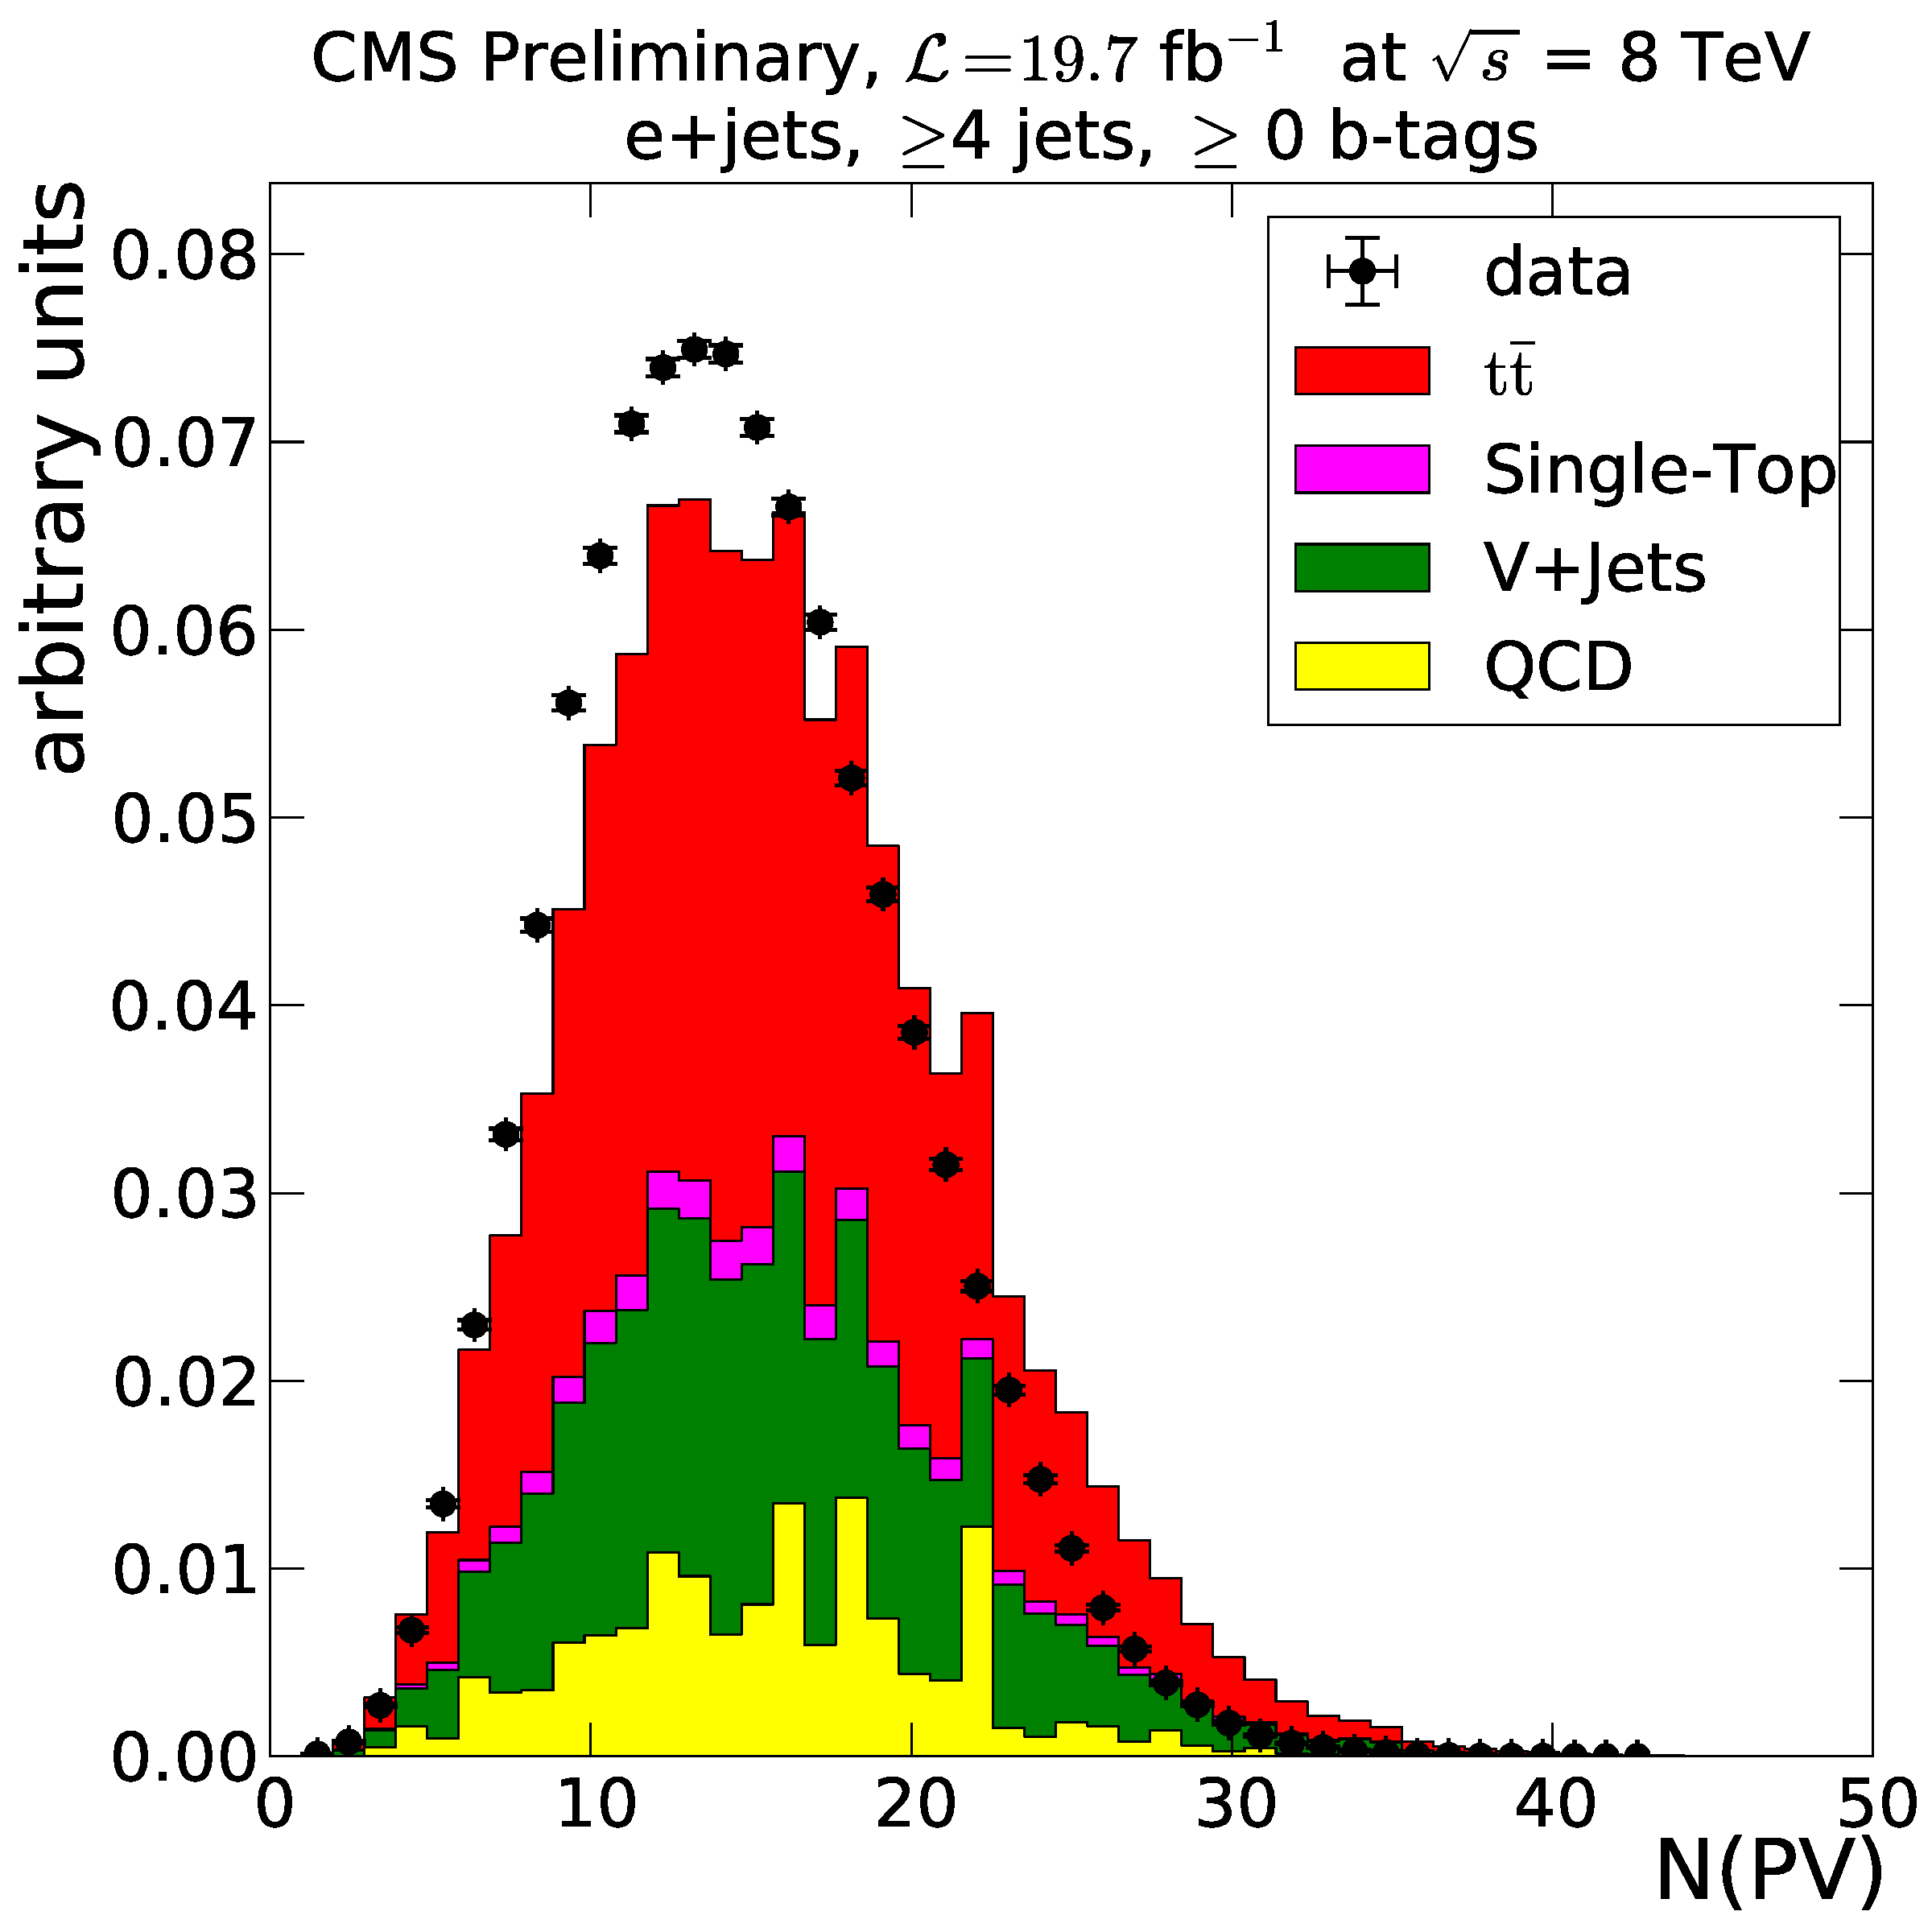
\includegraphics[width=0.50\textwidth]{vertices/EPlusJets_nVertex.pdf}}\hfill
	\subfloat[]{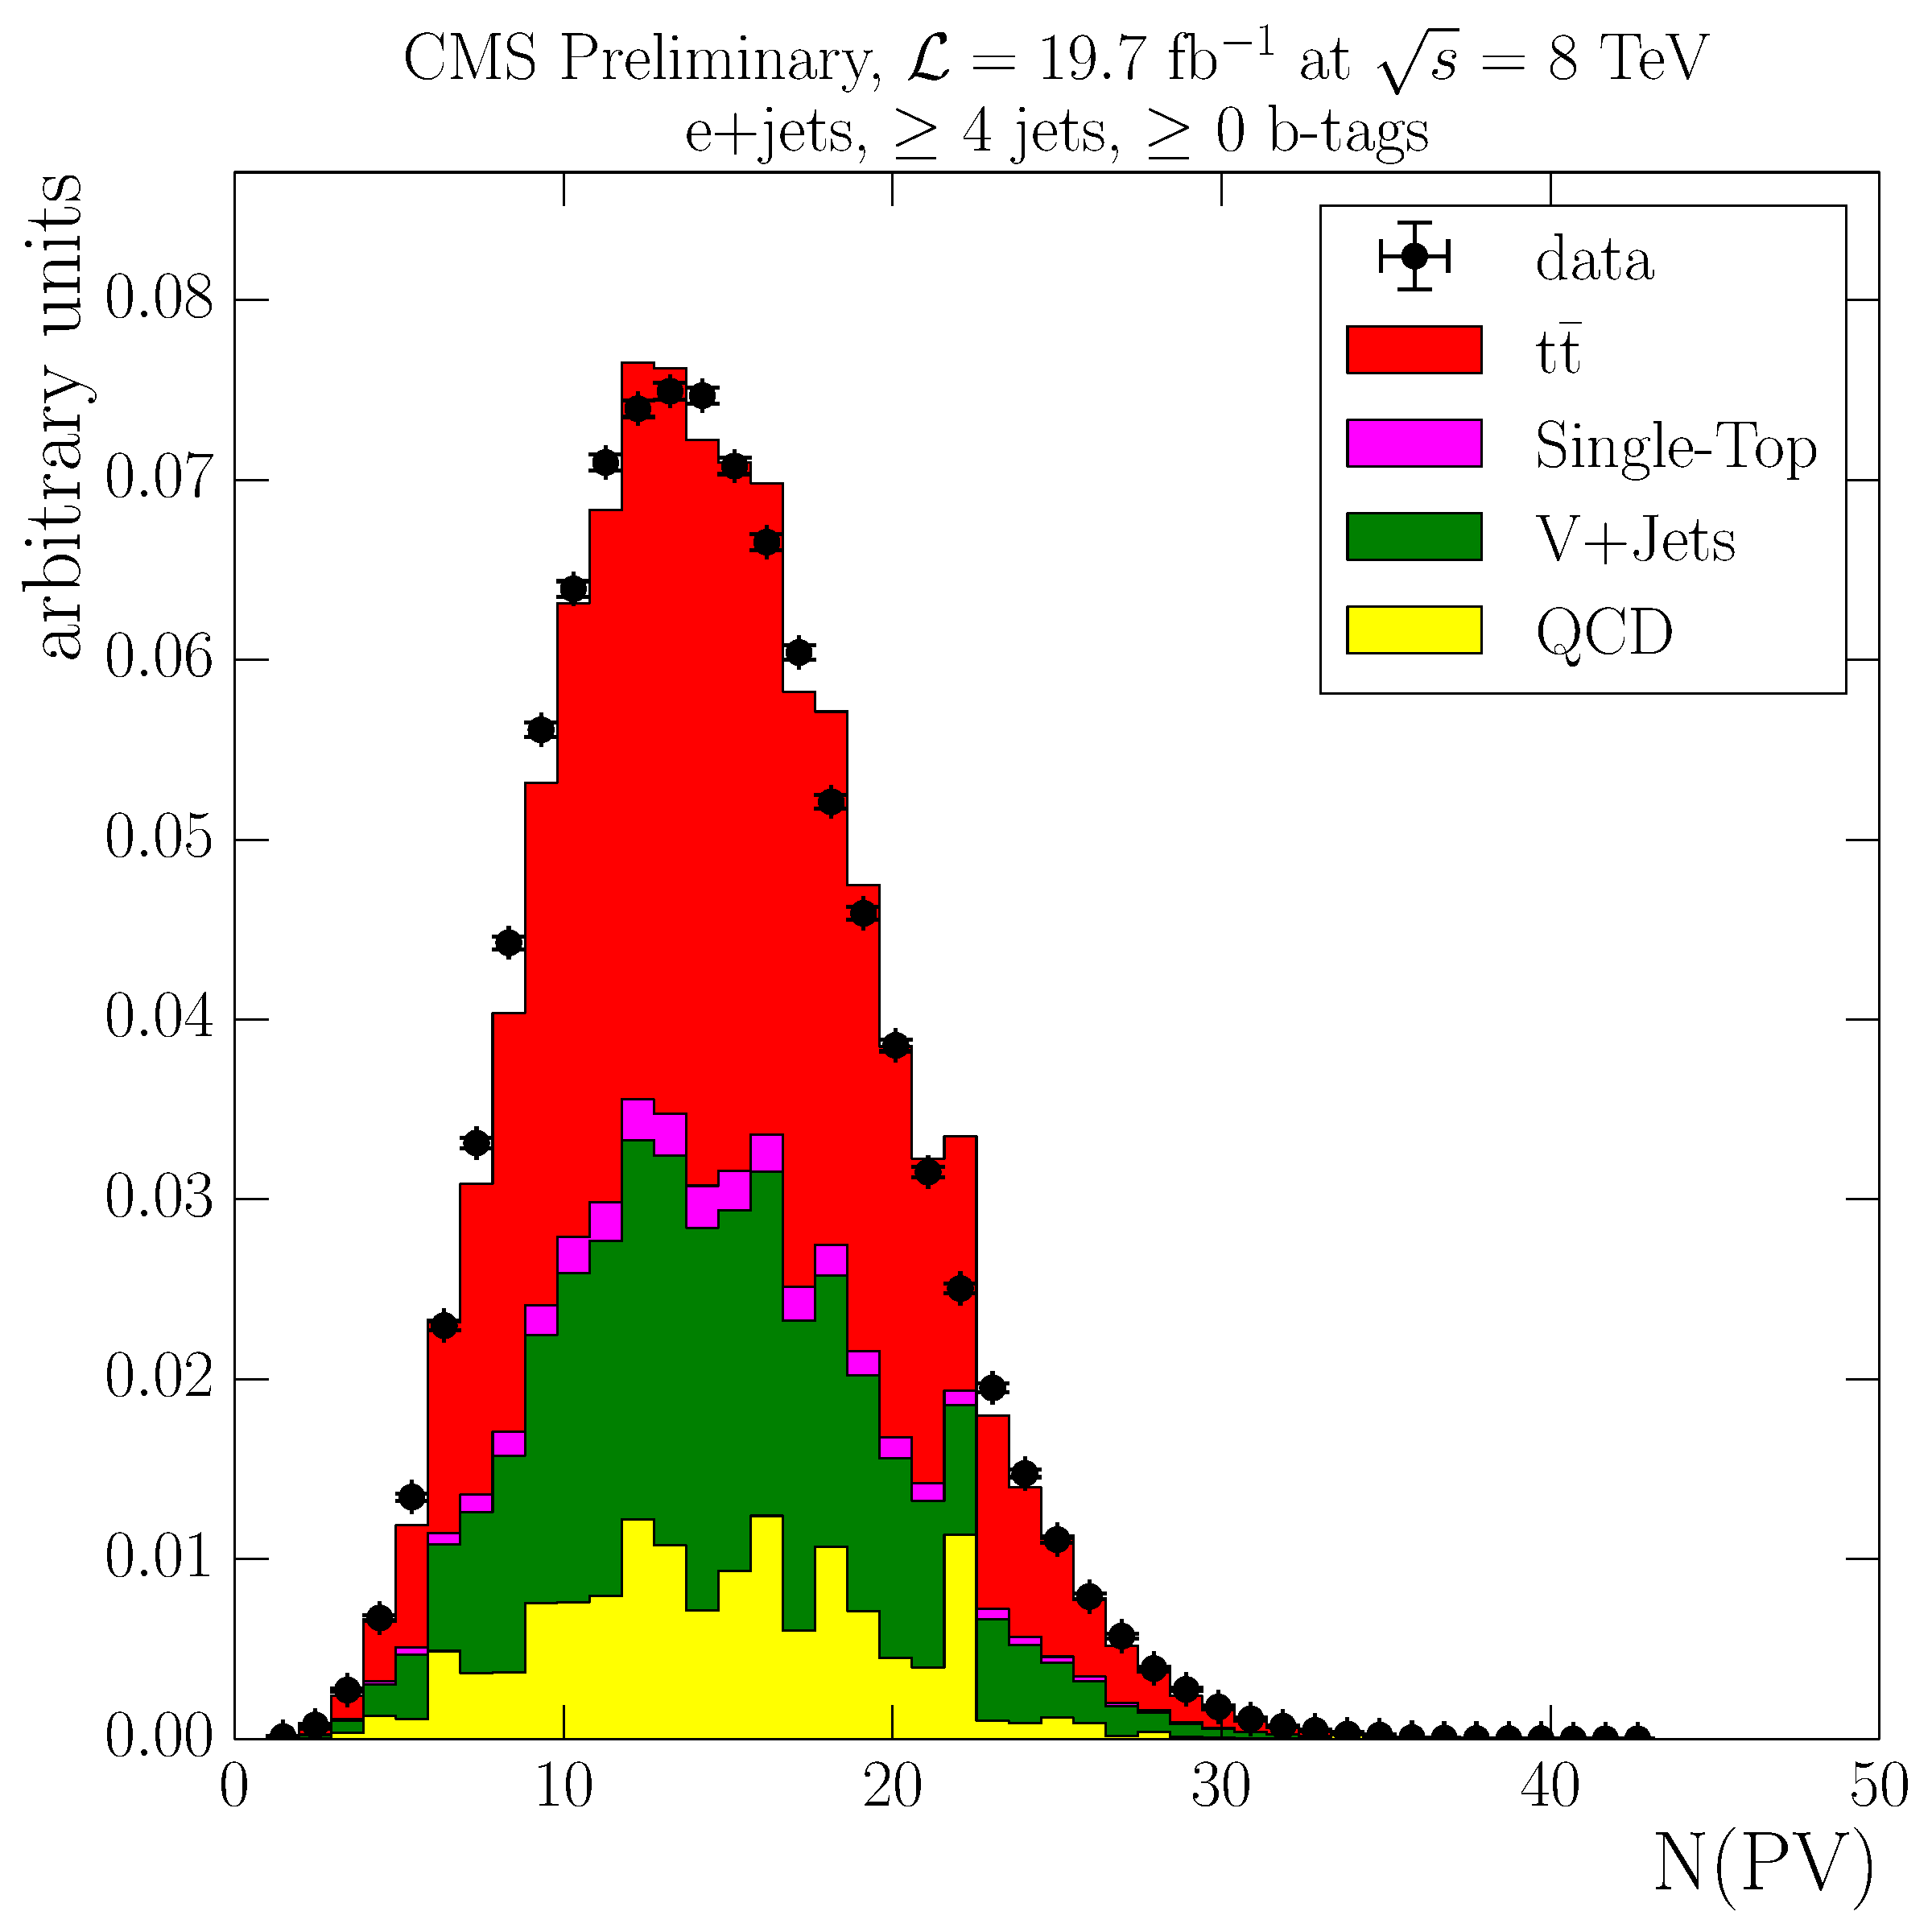
\includegraphics[width=0.50\textwidth]{vertices/EPlusJets_nVertex_reweighted.pdf}} \\
	\subfloat[]{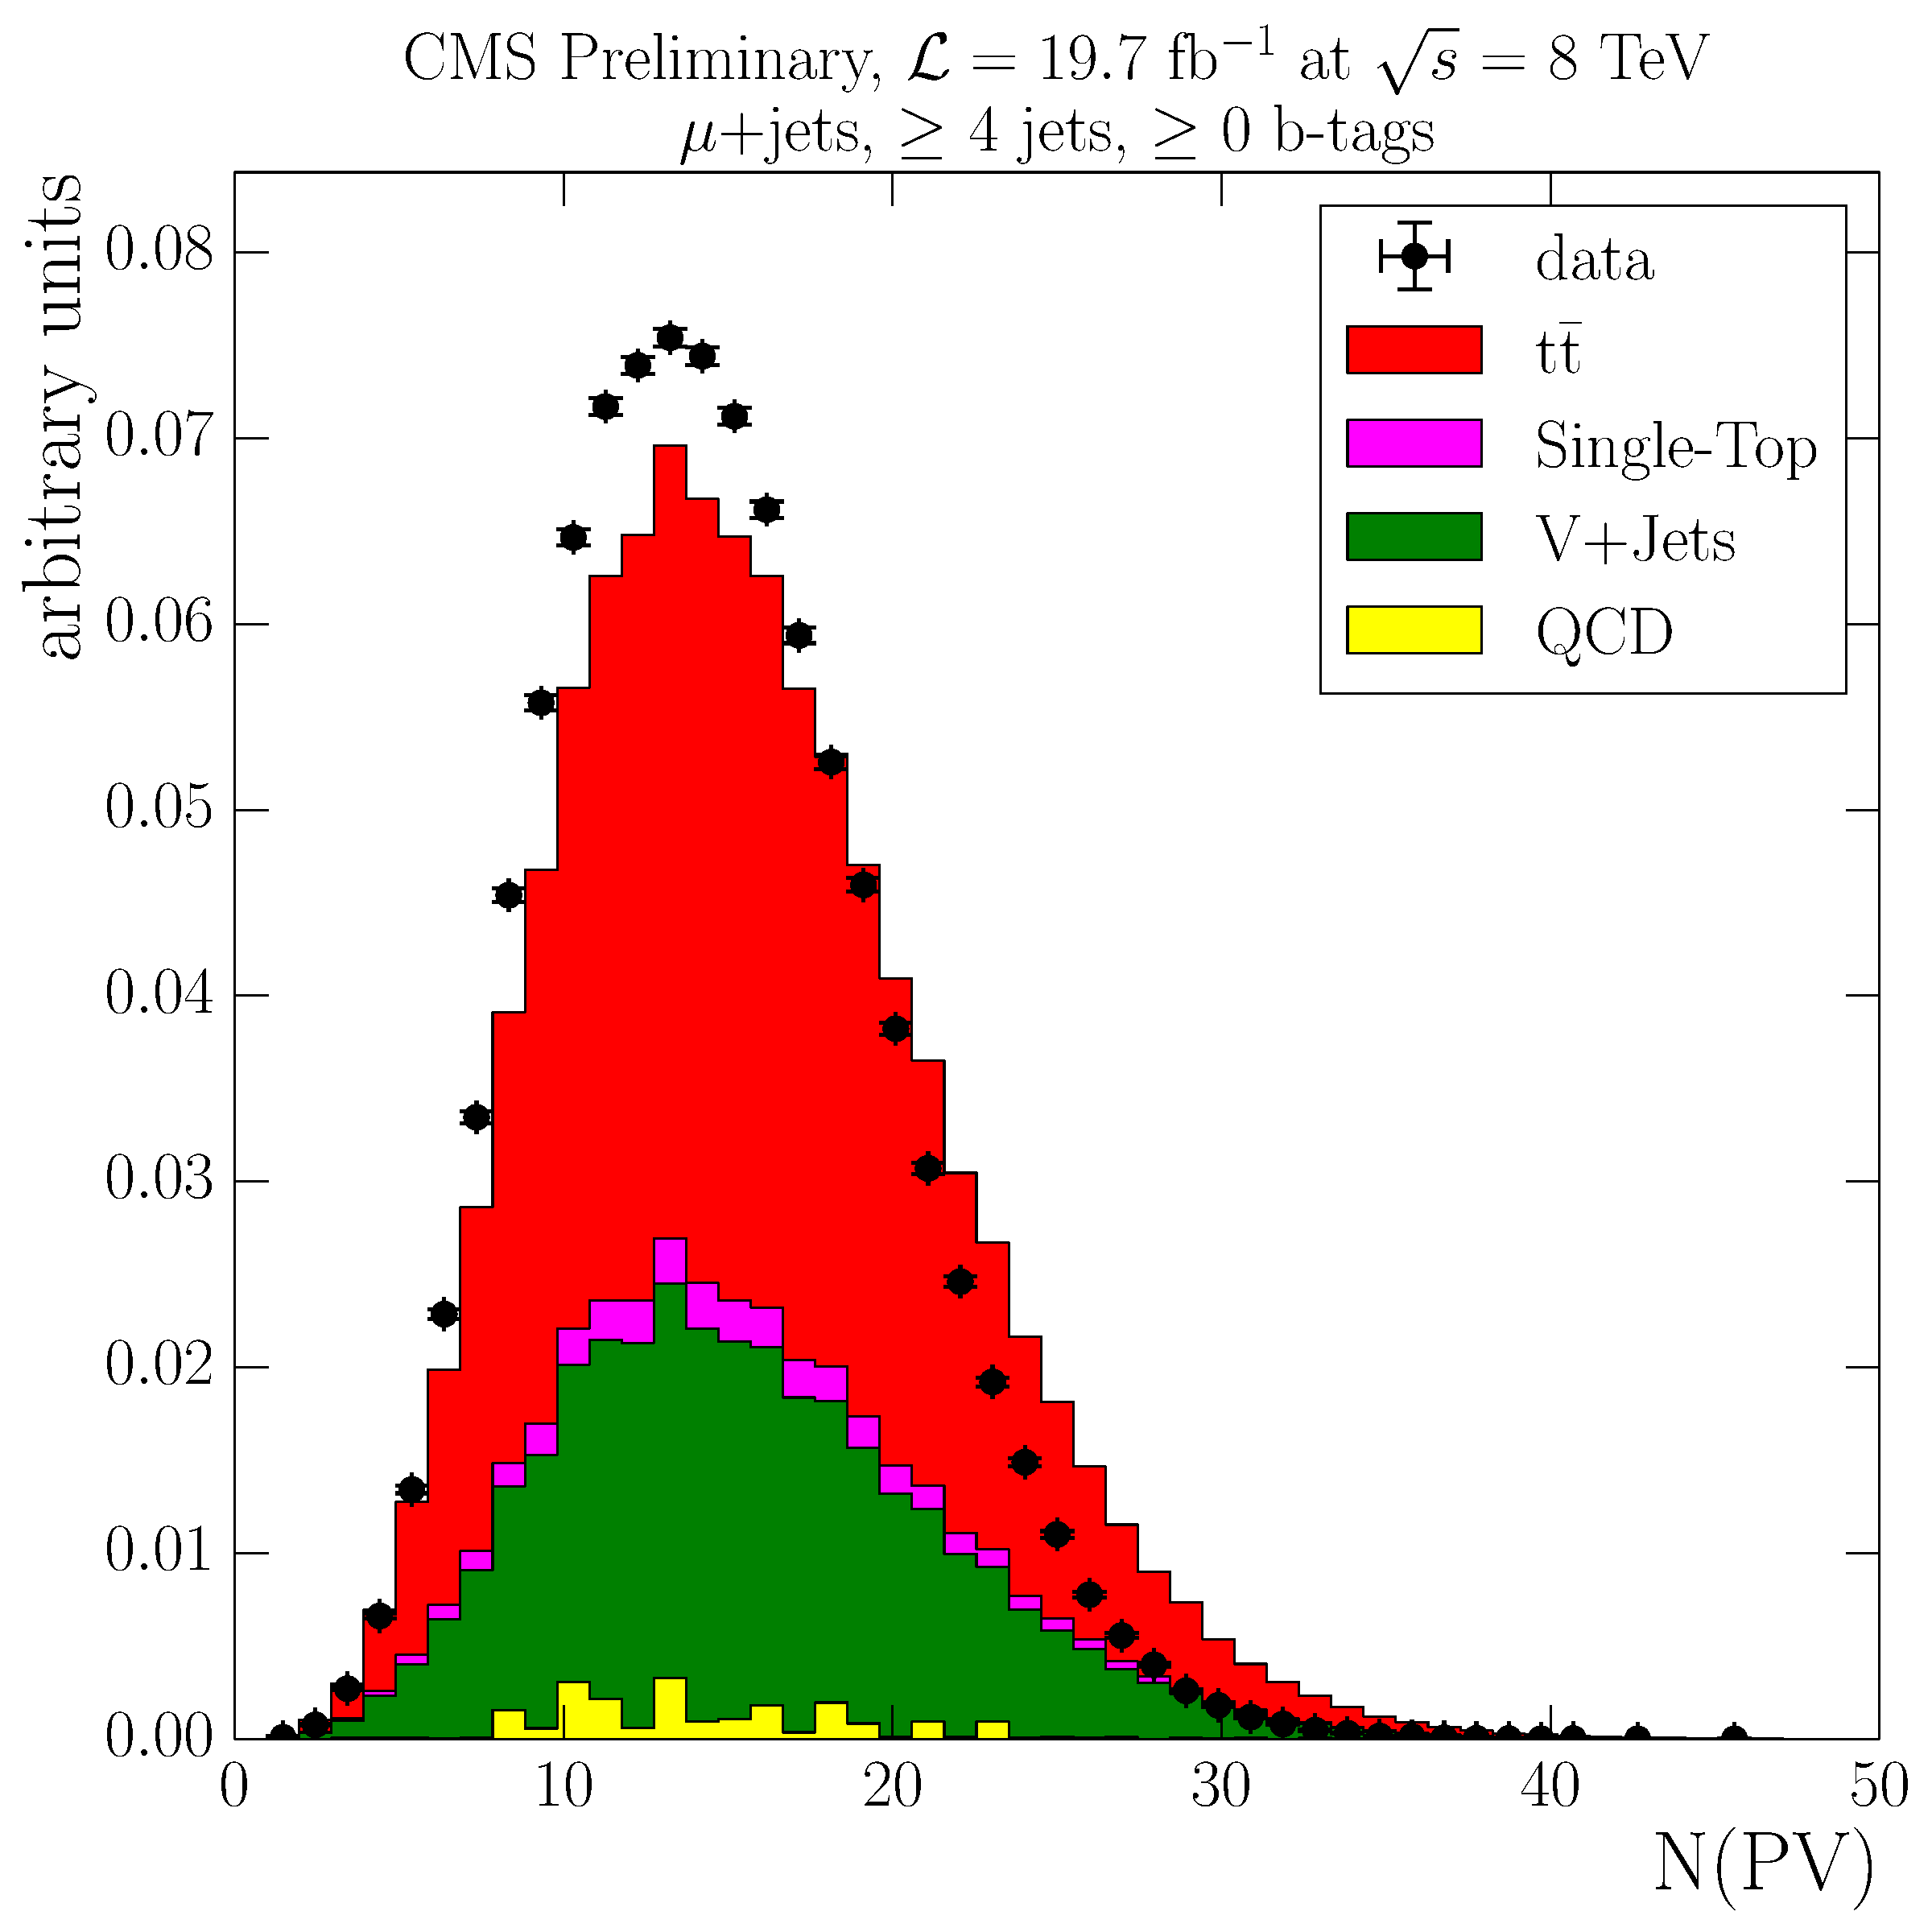
\includegraphics[width=0.50\textwidth]{vertices/MuPlusJets_nVertex.pdf}}\hfill
	\subfloat[]{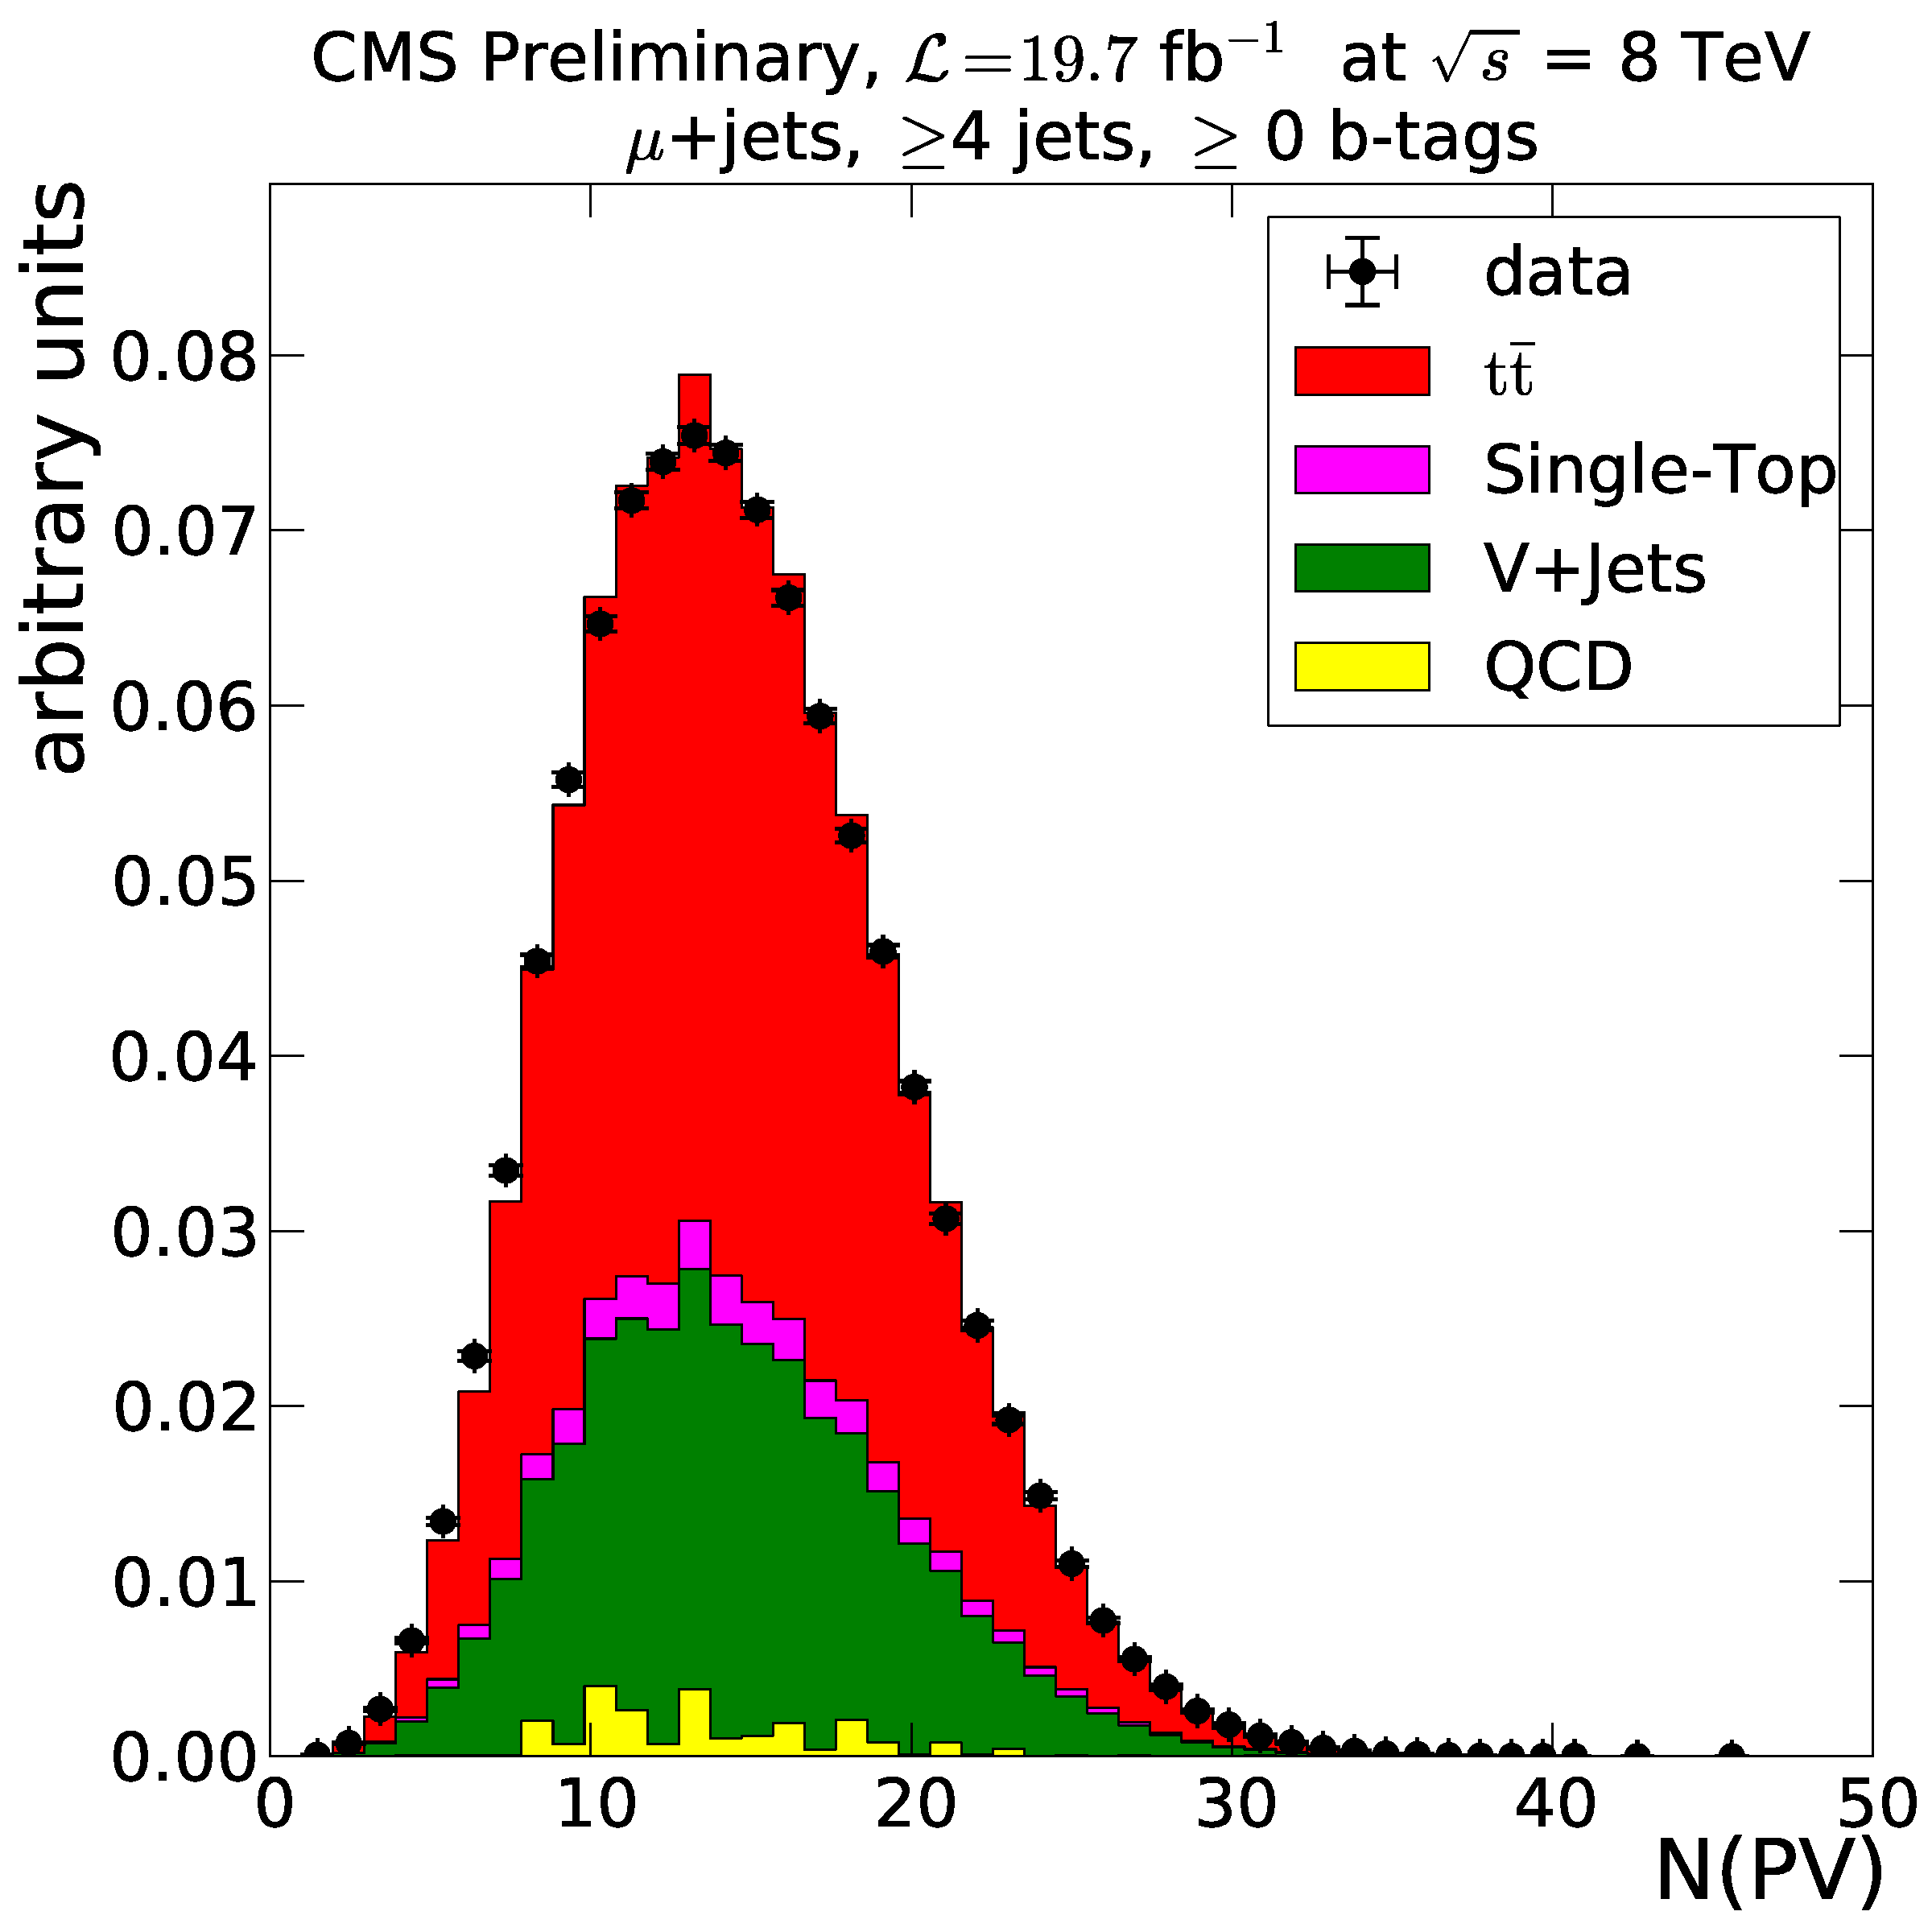
\includegraphics[width=0.50\textwidth]{vertices/MuPlusJets_nVertex_reweighted.pdf}}
	\caption{\label{fig:pileup_vertices}
    Number of reconstructed vertices per event before (left) and after pile-up reweighting (right) in the electron
    channel (top) and in the muon channel (bottom). Both data and sum of the MC samples are normalised to unit area.}
    %QCD is estimated from MC here. Possible to fix/remove?
\end{center}
\end{figure}

\begin{figure}[!htpb]
\begin{center}
	\subfloat[]{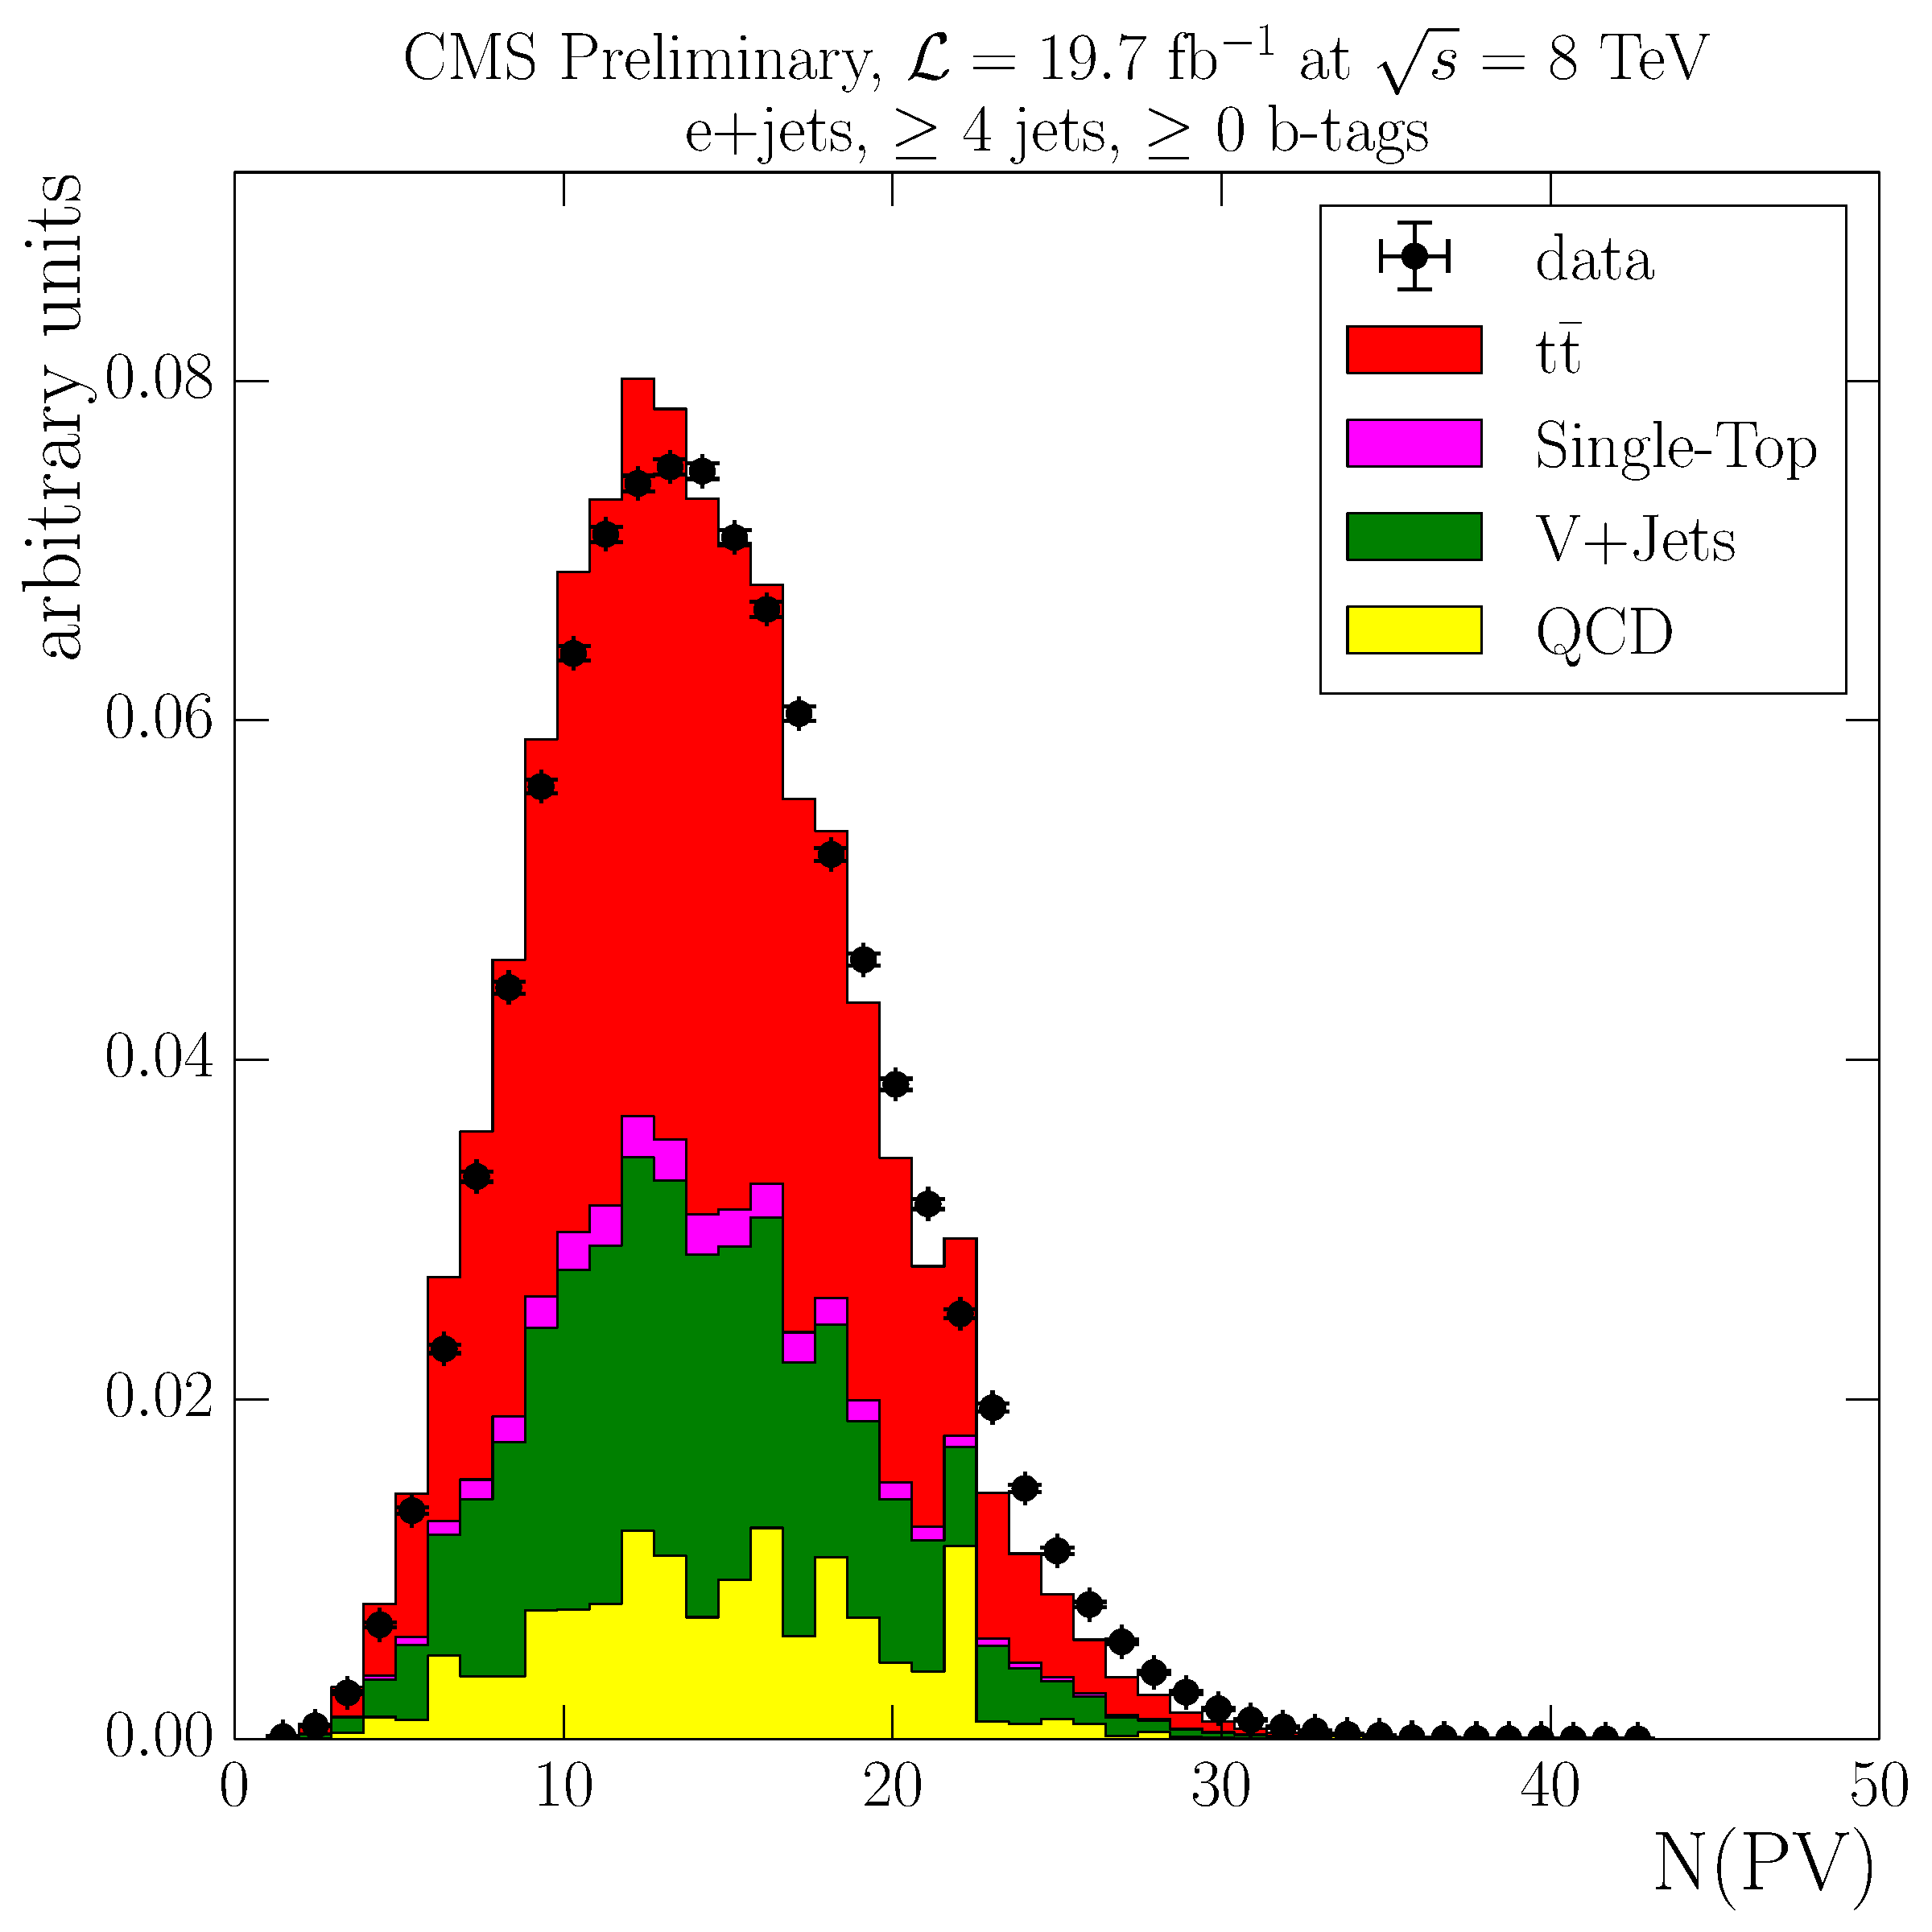
\includegraphics[width=0.50\textwidth]{vertices/EPlusJets_nVertex_reweighted_PU_down.pdf}}\hfill
	\subfloat[]{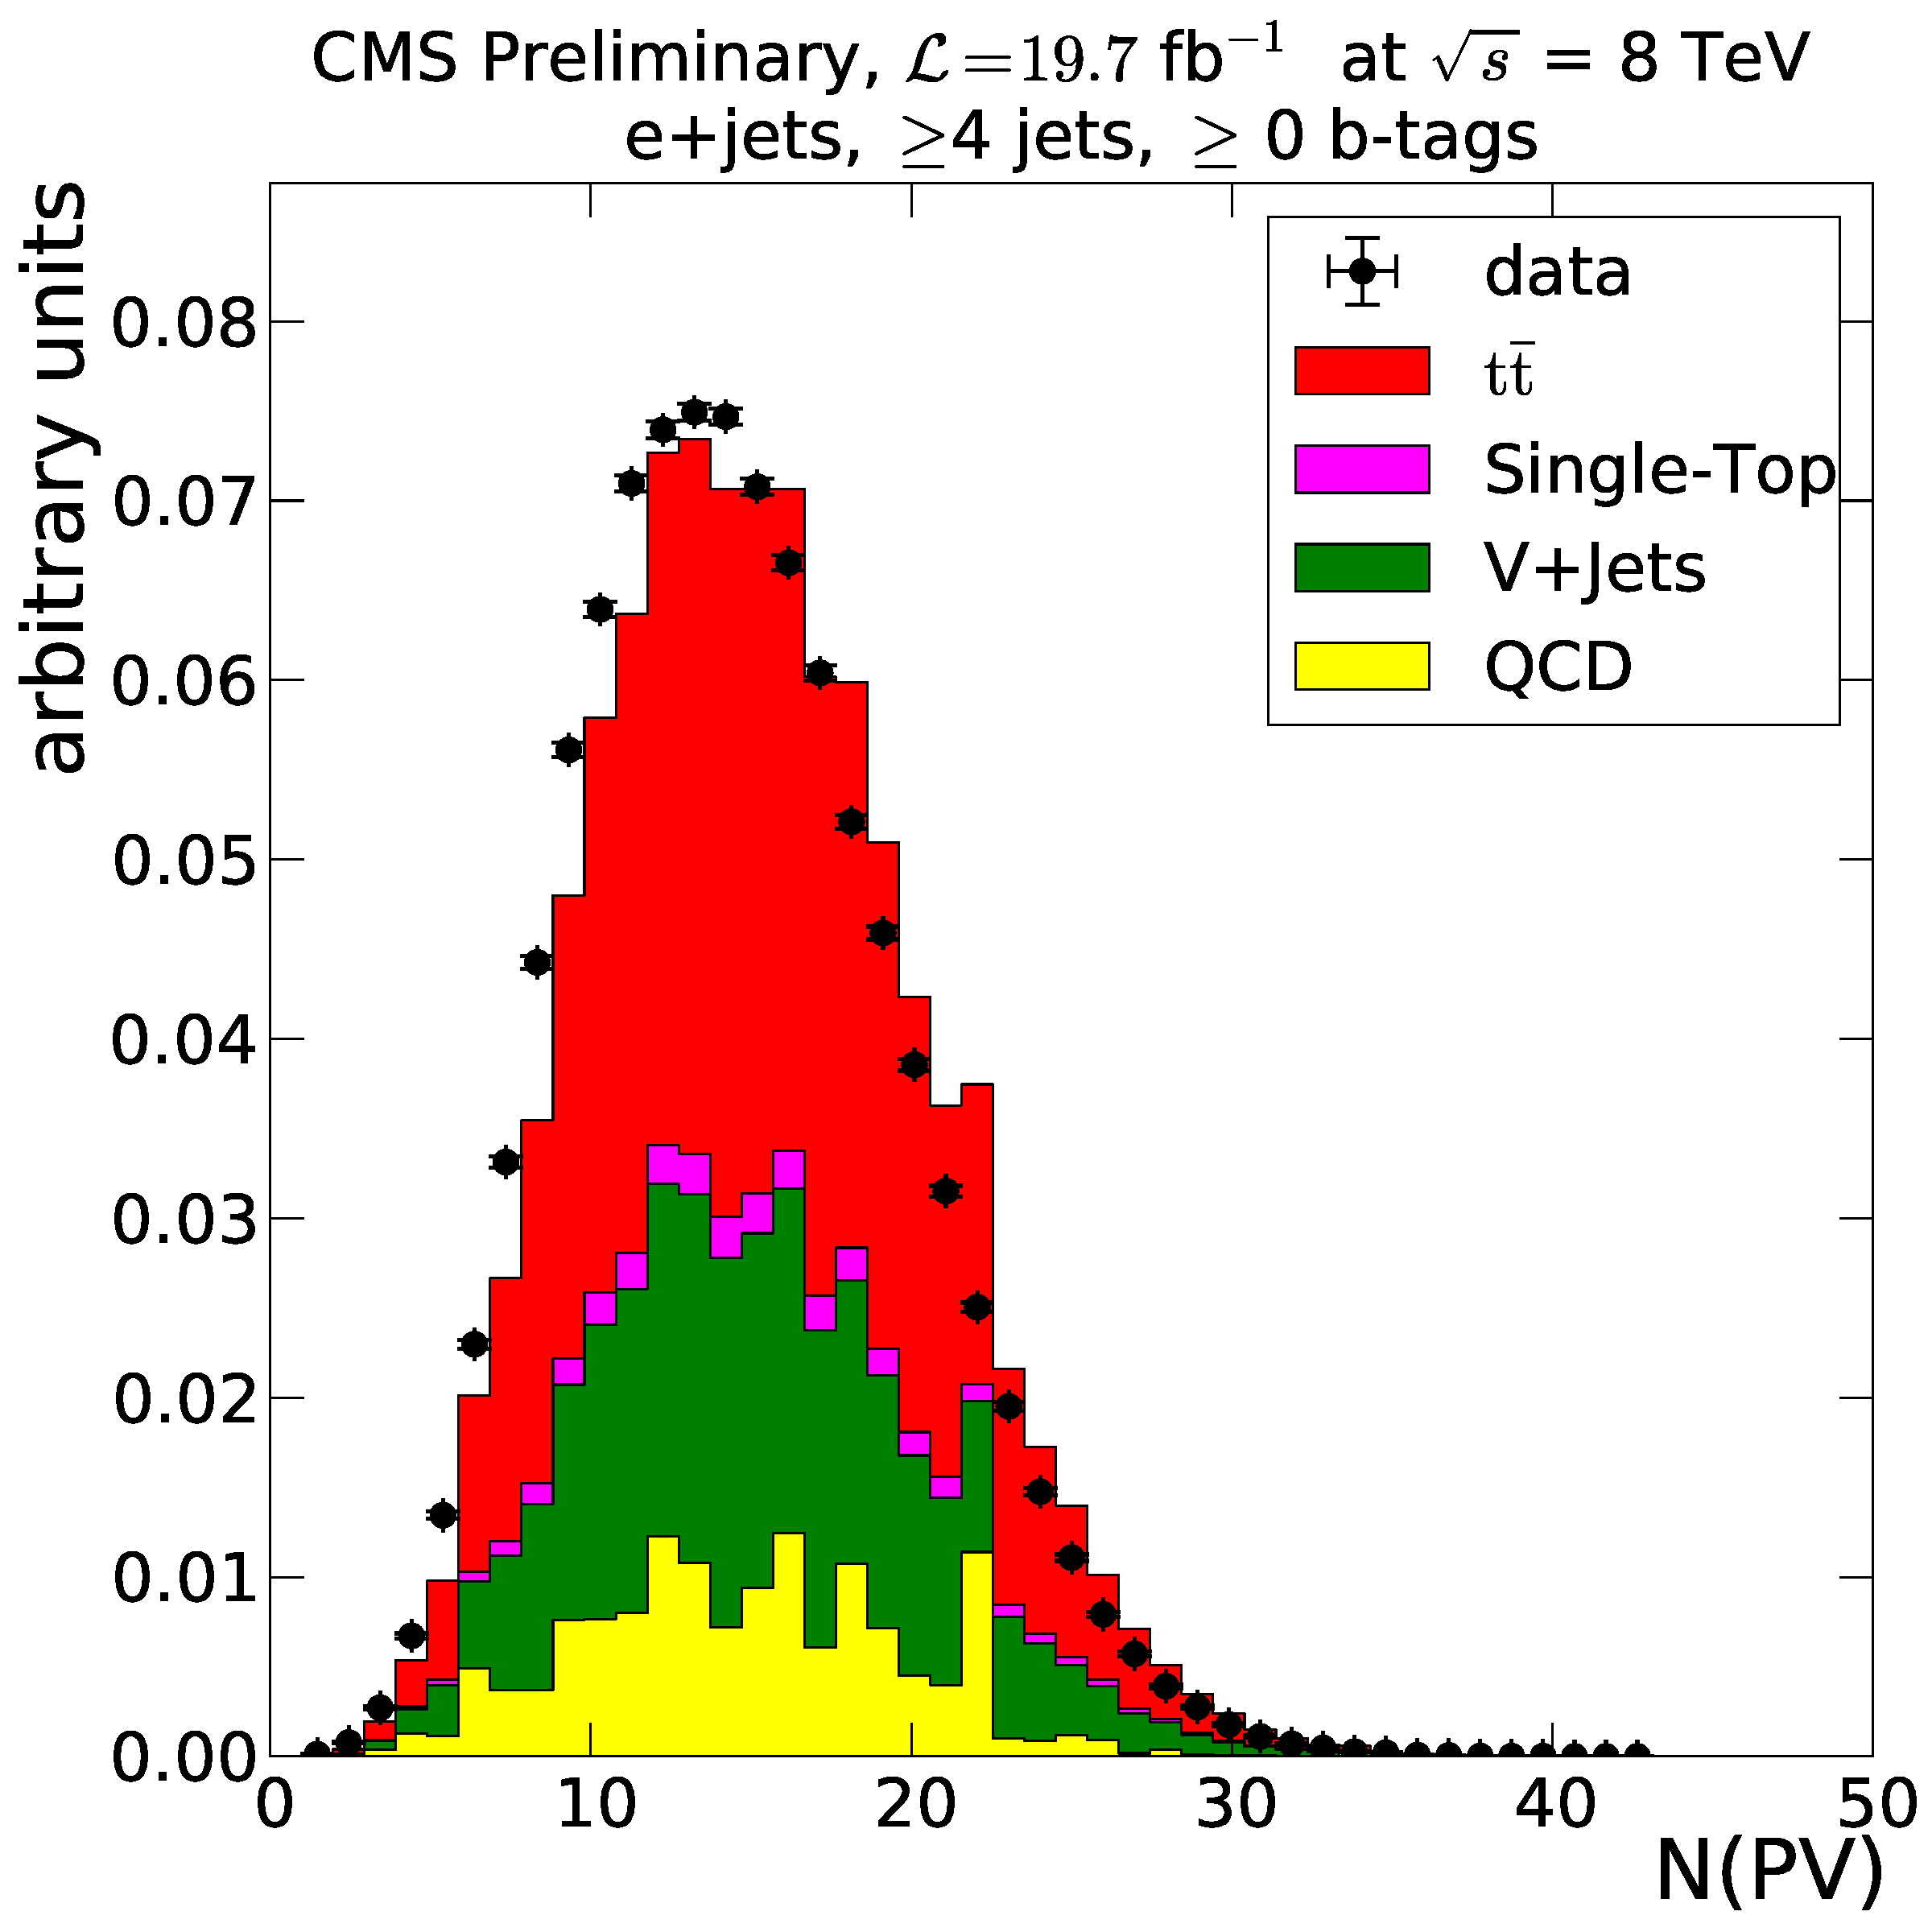
\includegraphics[width=0.50\textwidth]{vertices/EPlusJets_nVertex_reweighted_PU_up.pdf}} \\
	\subfloat[]{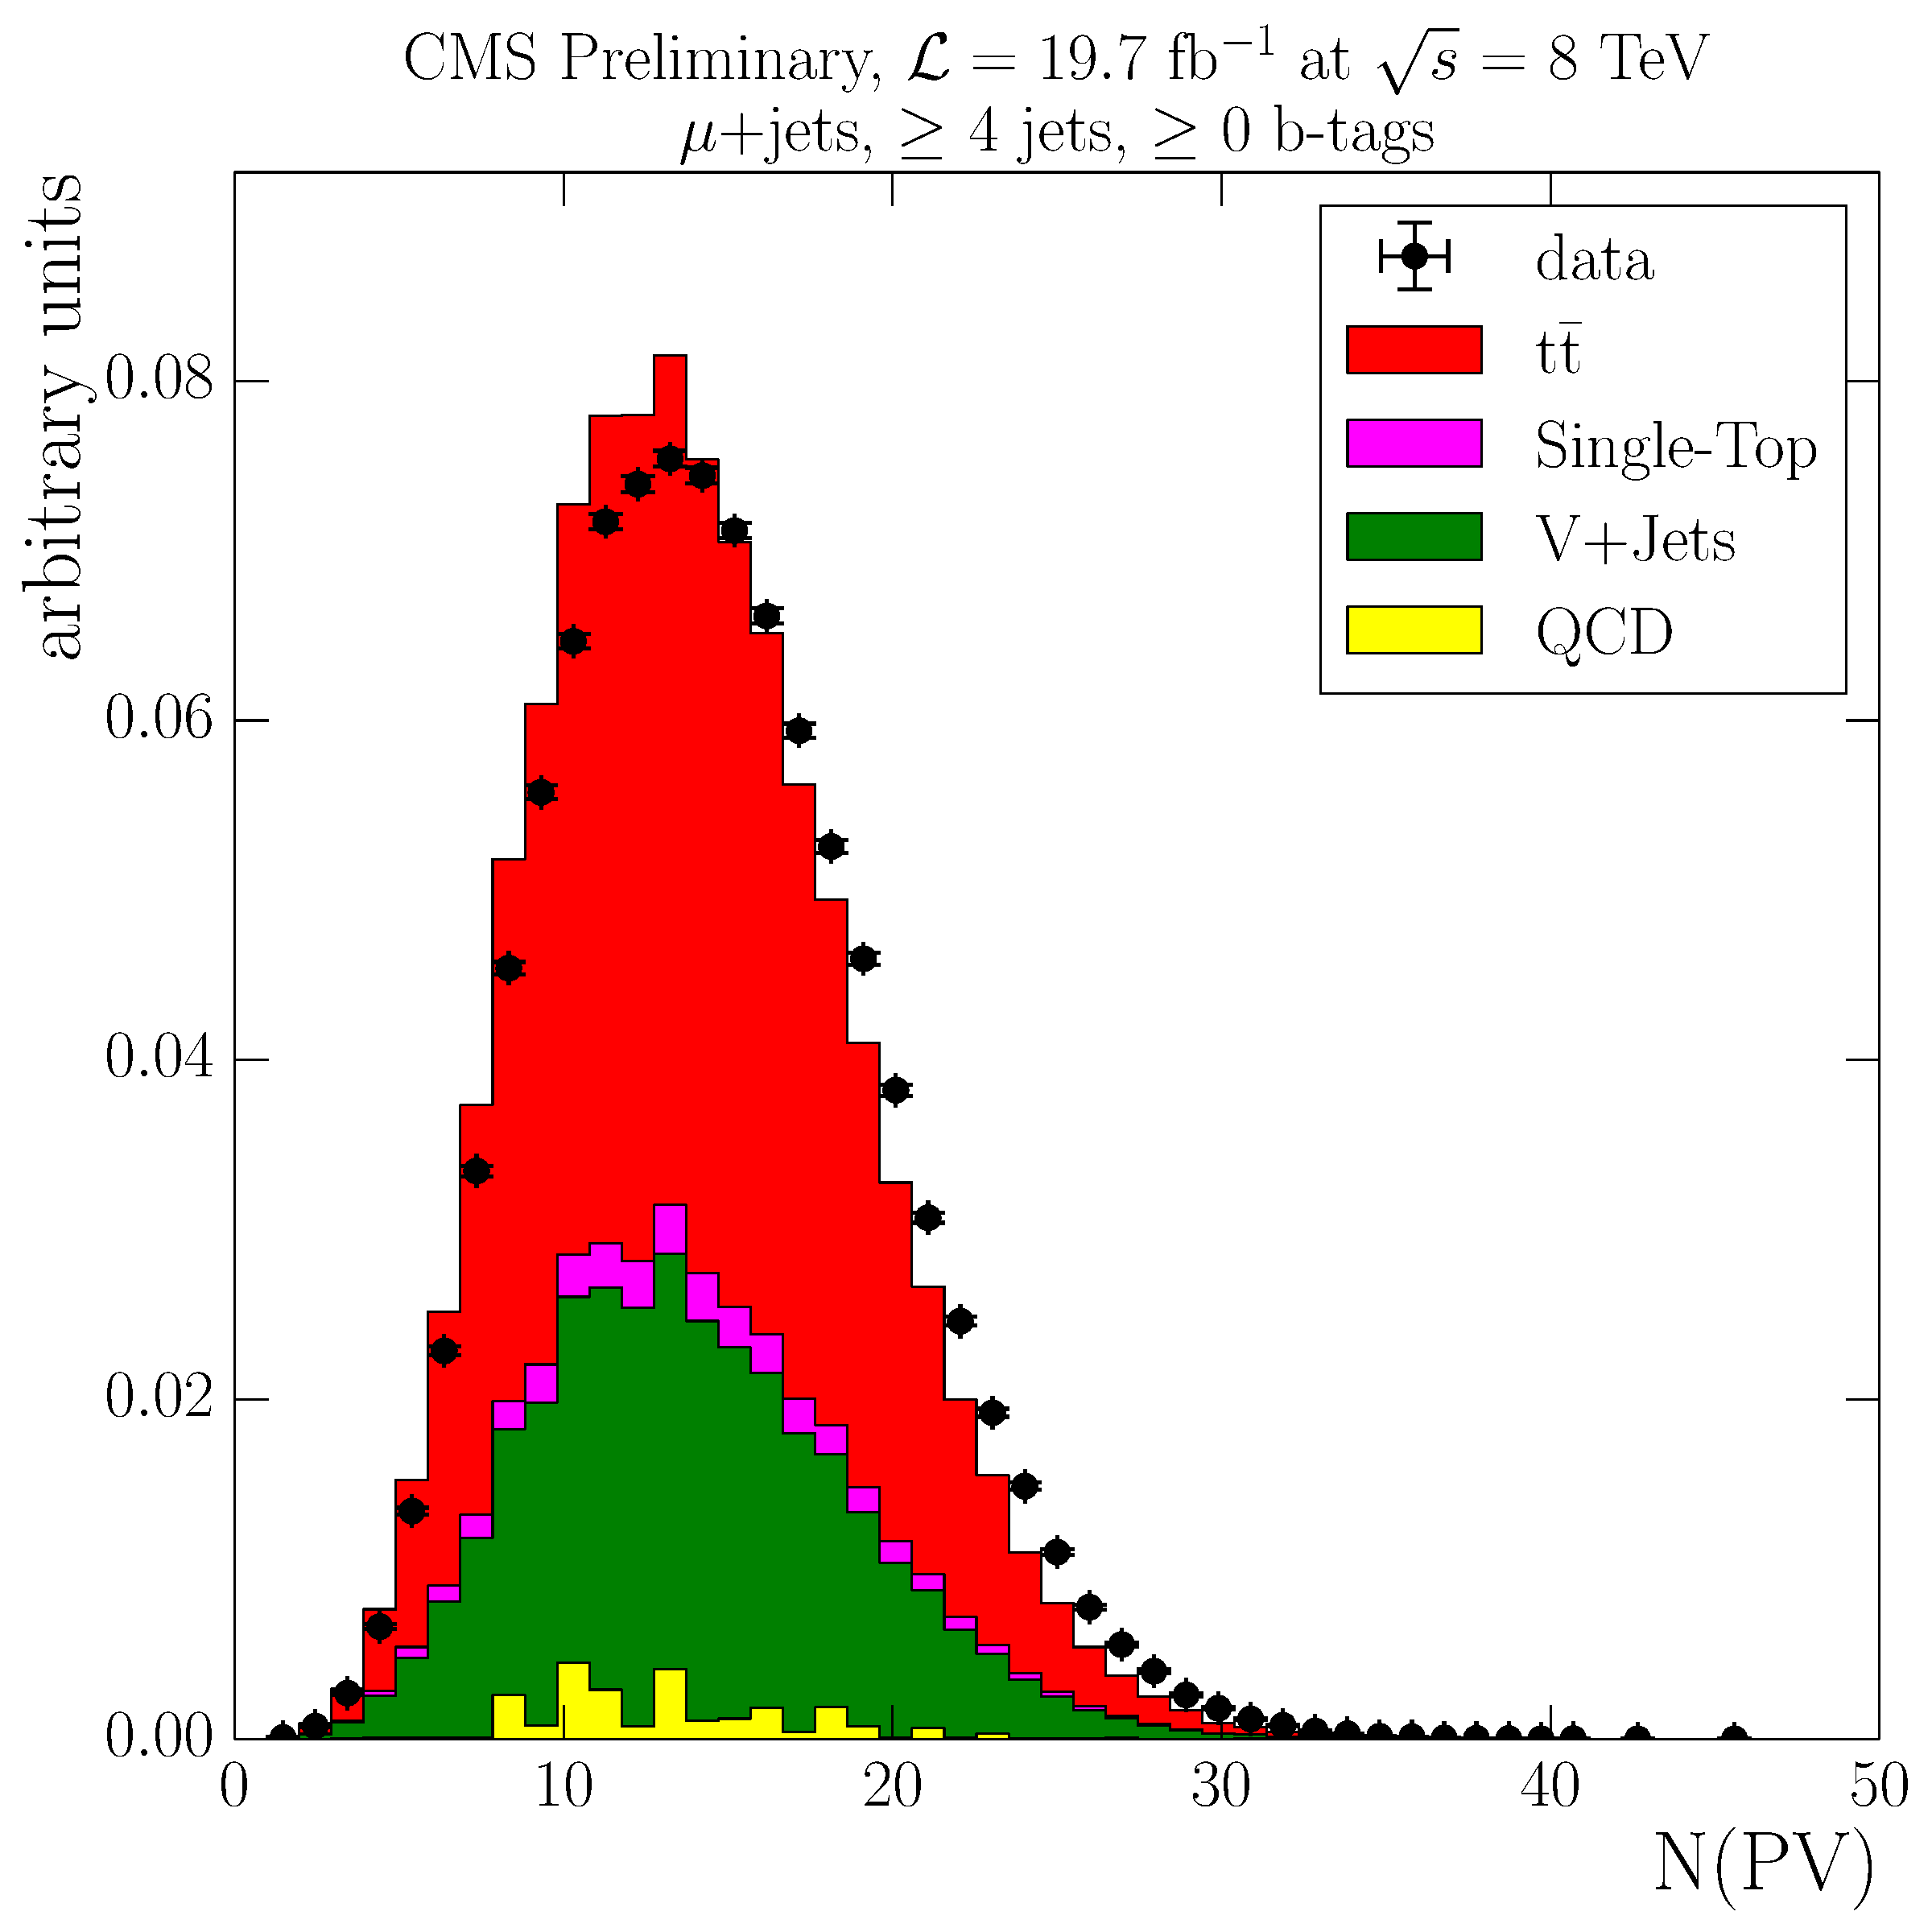
\includegraphics[width=0.50\textwidth]{vertices/MuPlusJets_nVertex_reweighted_PU_down.pdf}}\hfill
	\subfloat[]{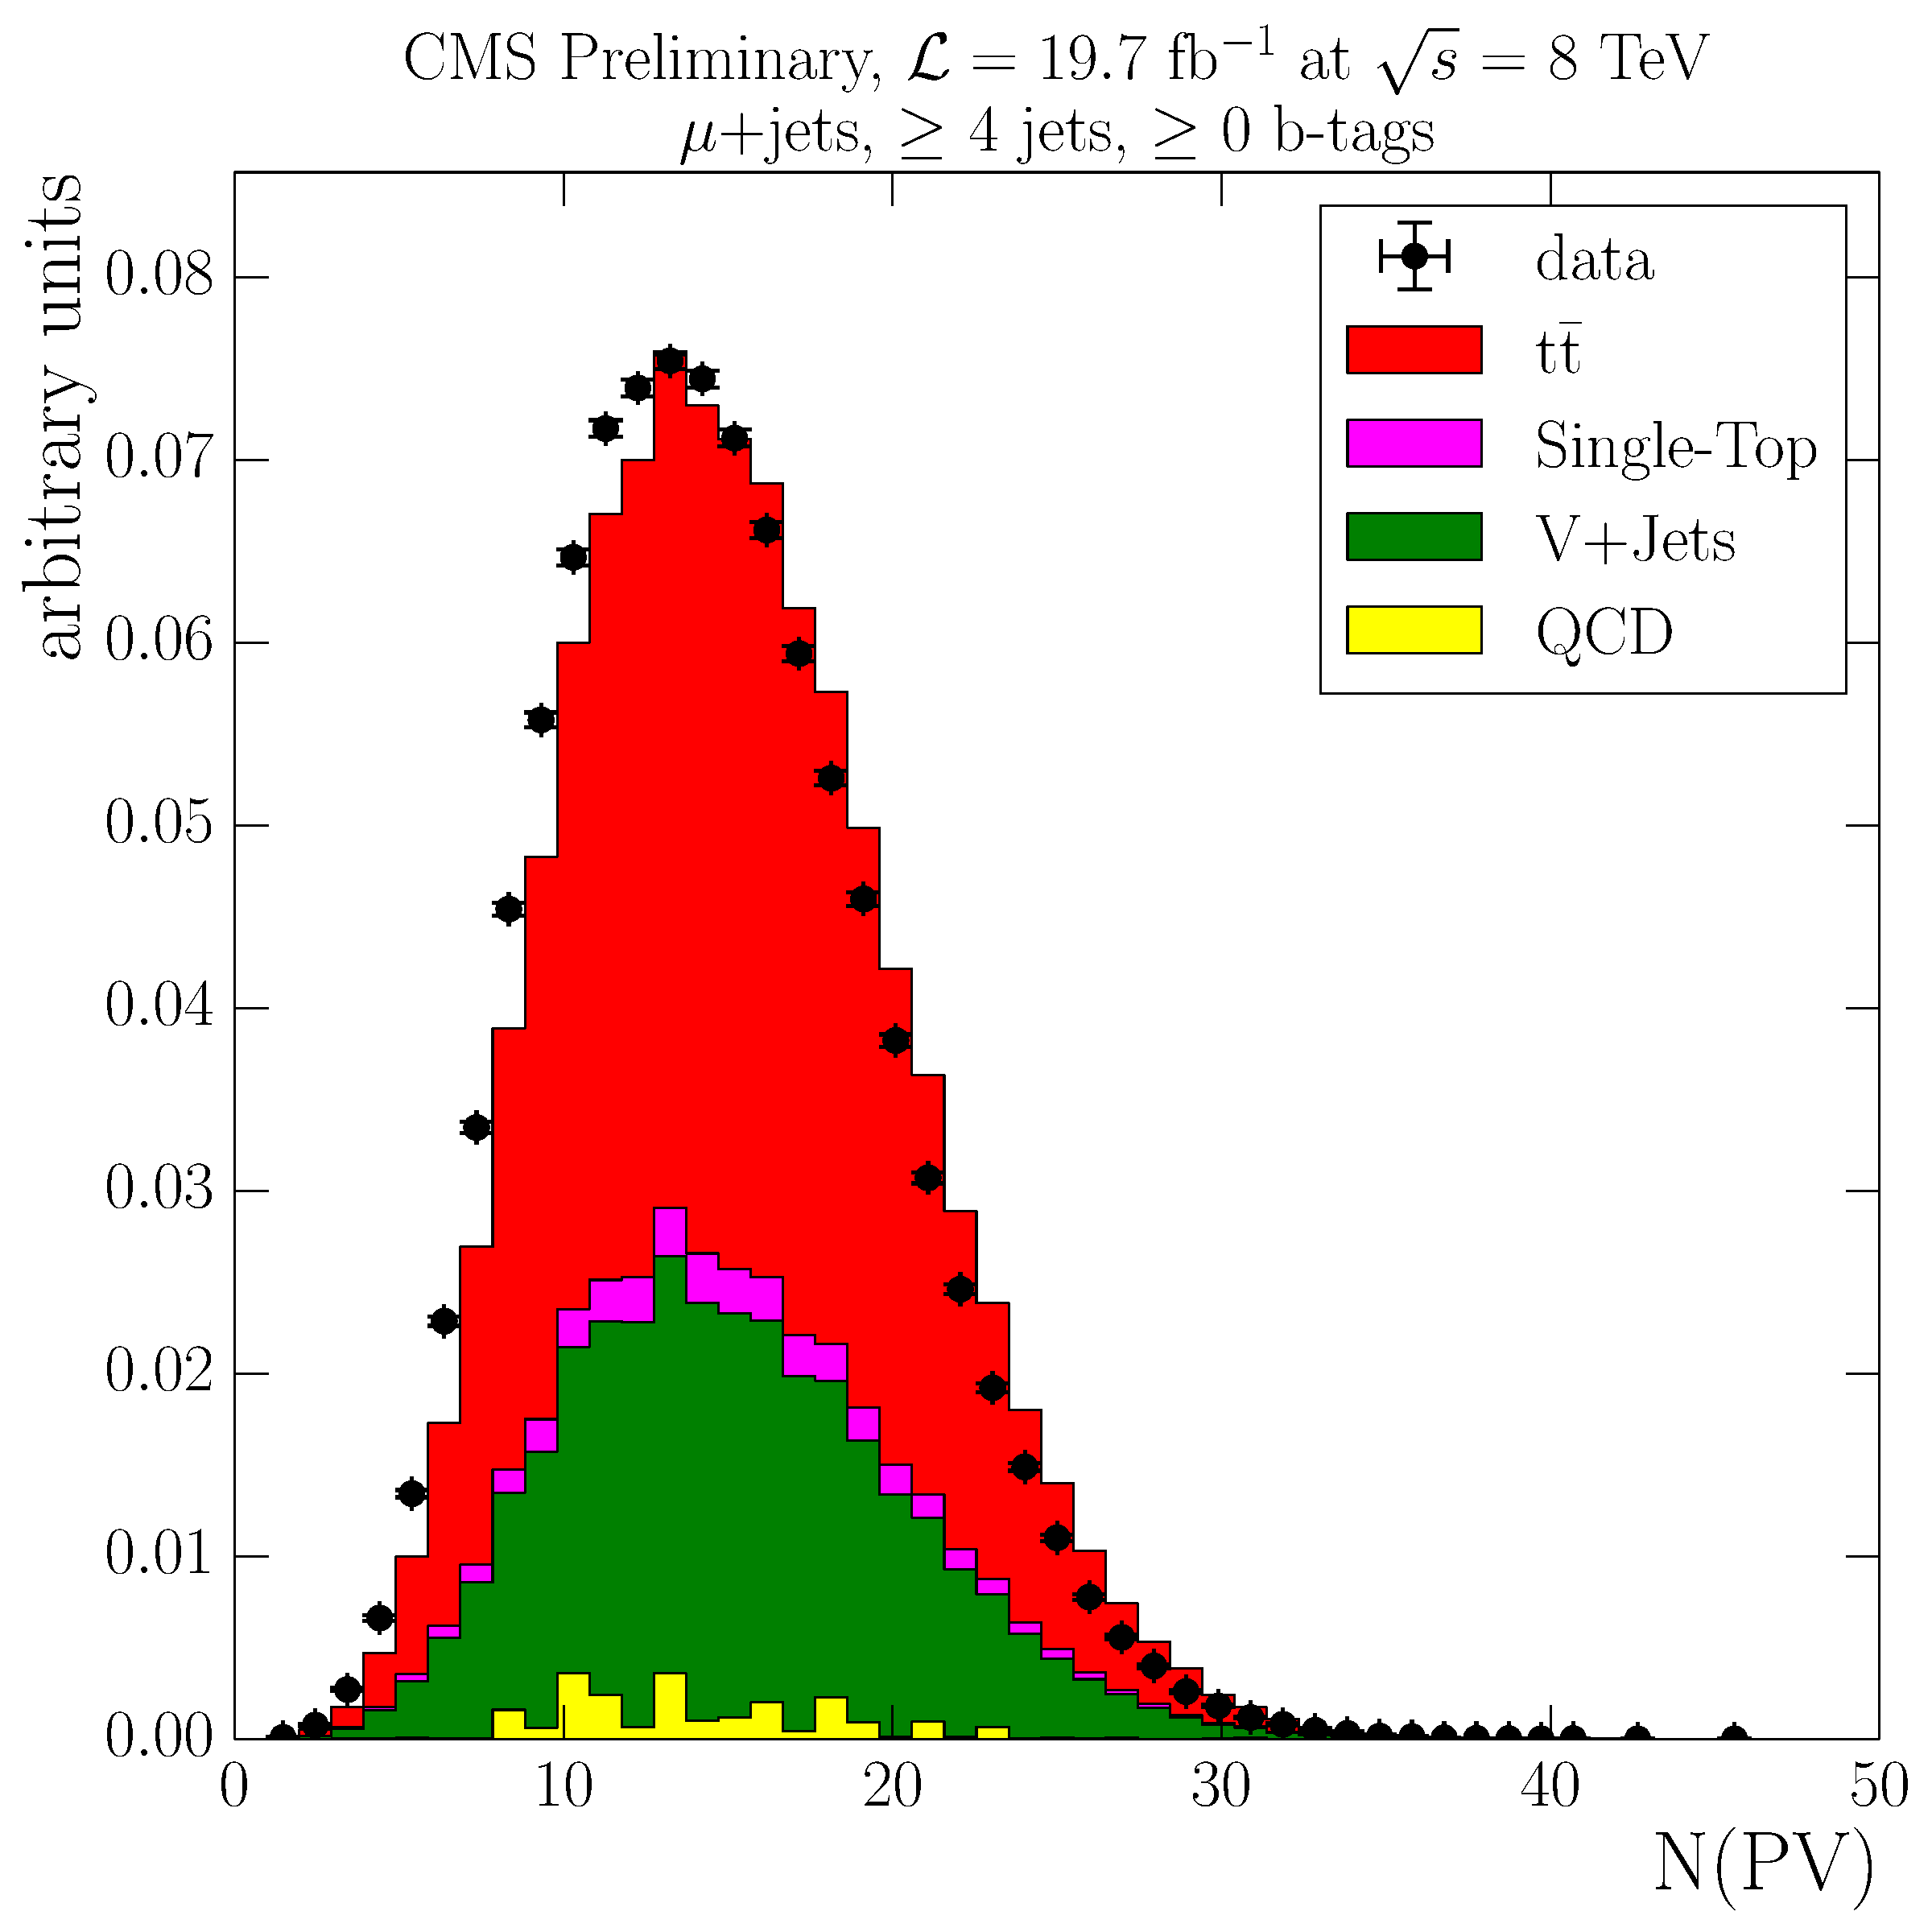
\includegraphics[width=0.50\textwidth]{vertices/MuPlusJets_nVertex_reweighted_PU_up.pdf}}
	\caption{\label{fig:pileup_vertices_variations}
    Number of reconstructed vertices per event for the $-\sigma$ (left) and the $+\sigma$ variations (right) of
    the pile-up reweighting procedure for the electron channel (top) and the muon channel (bottom).}
\end{center}
\end{figure}


\subsection{b-tagging corrections}
\label{ss_xsection:btagging_corrections}

\begin{figure}[!htpb]
\begin{center}
	\subfloat[]{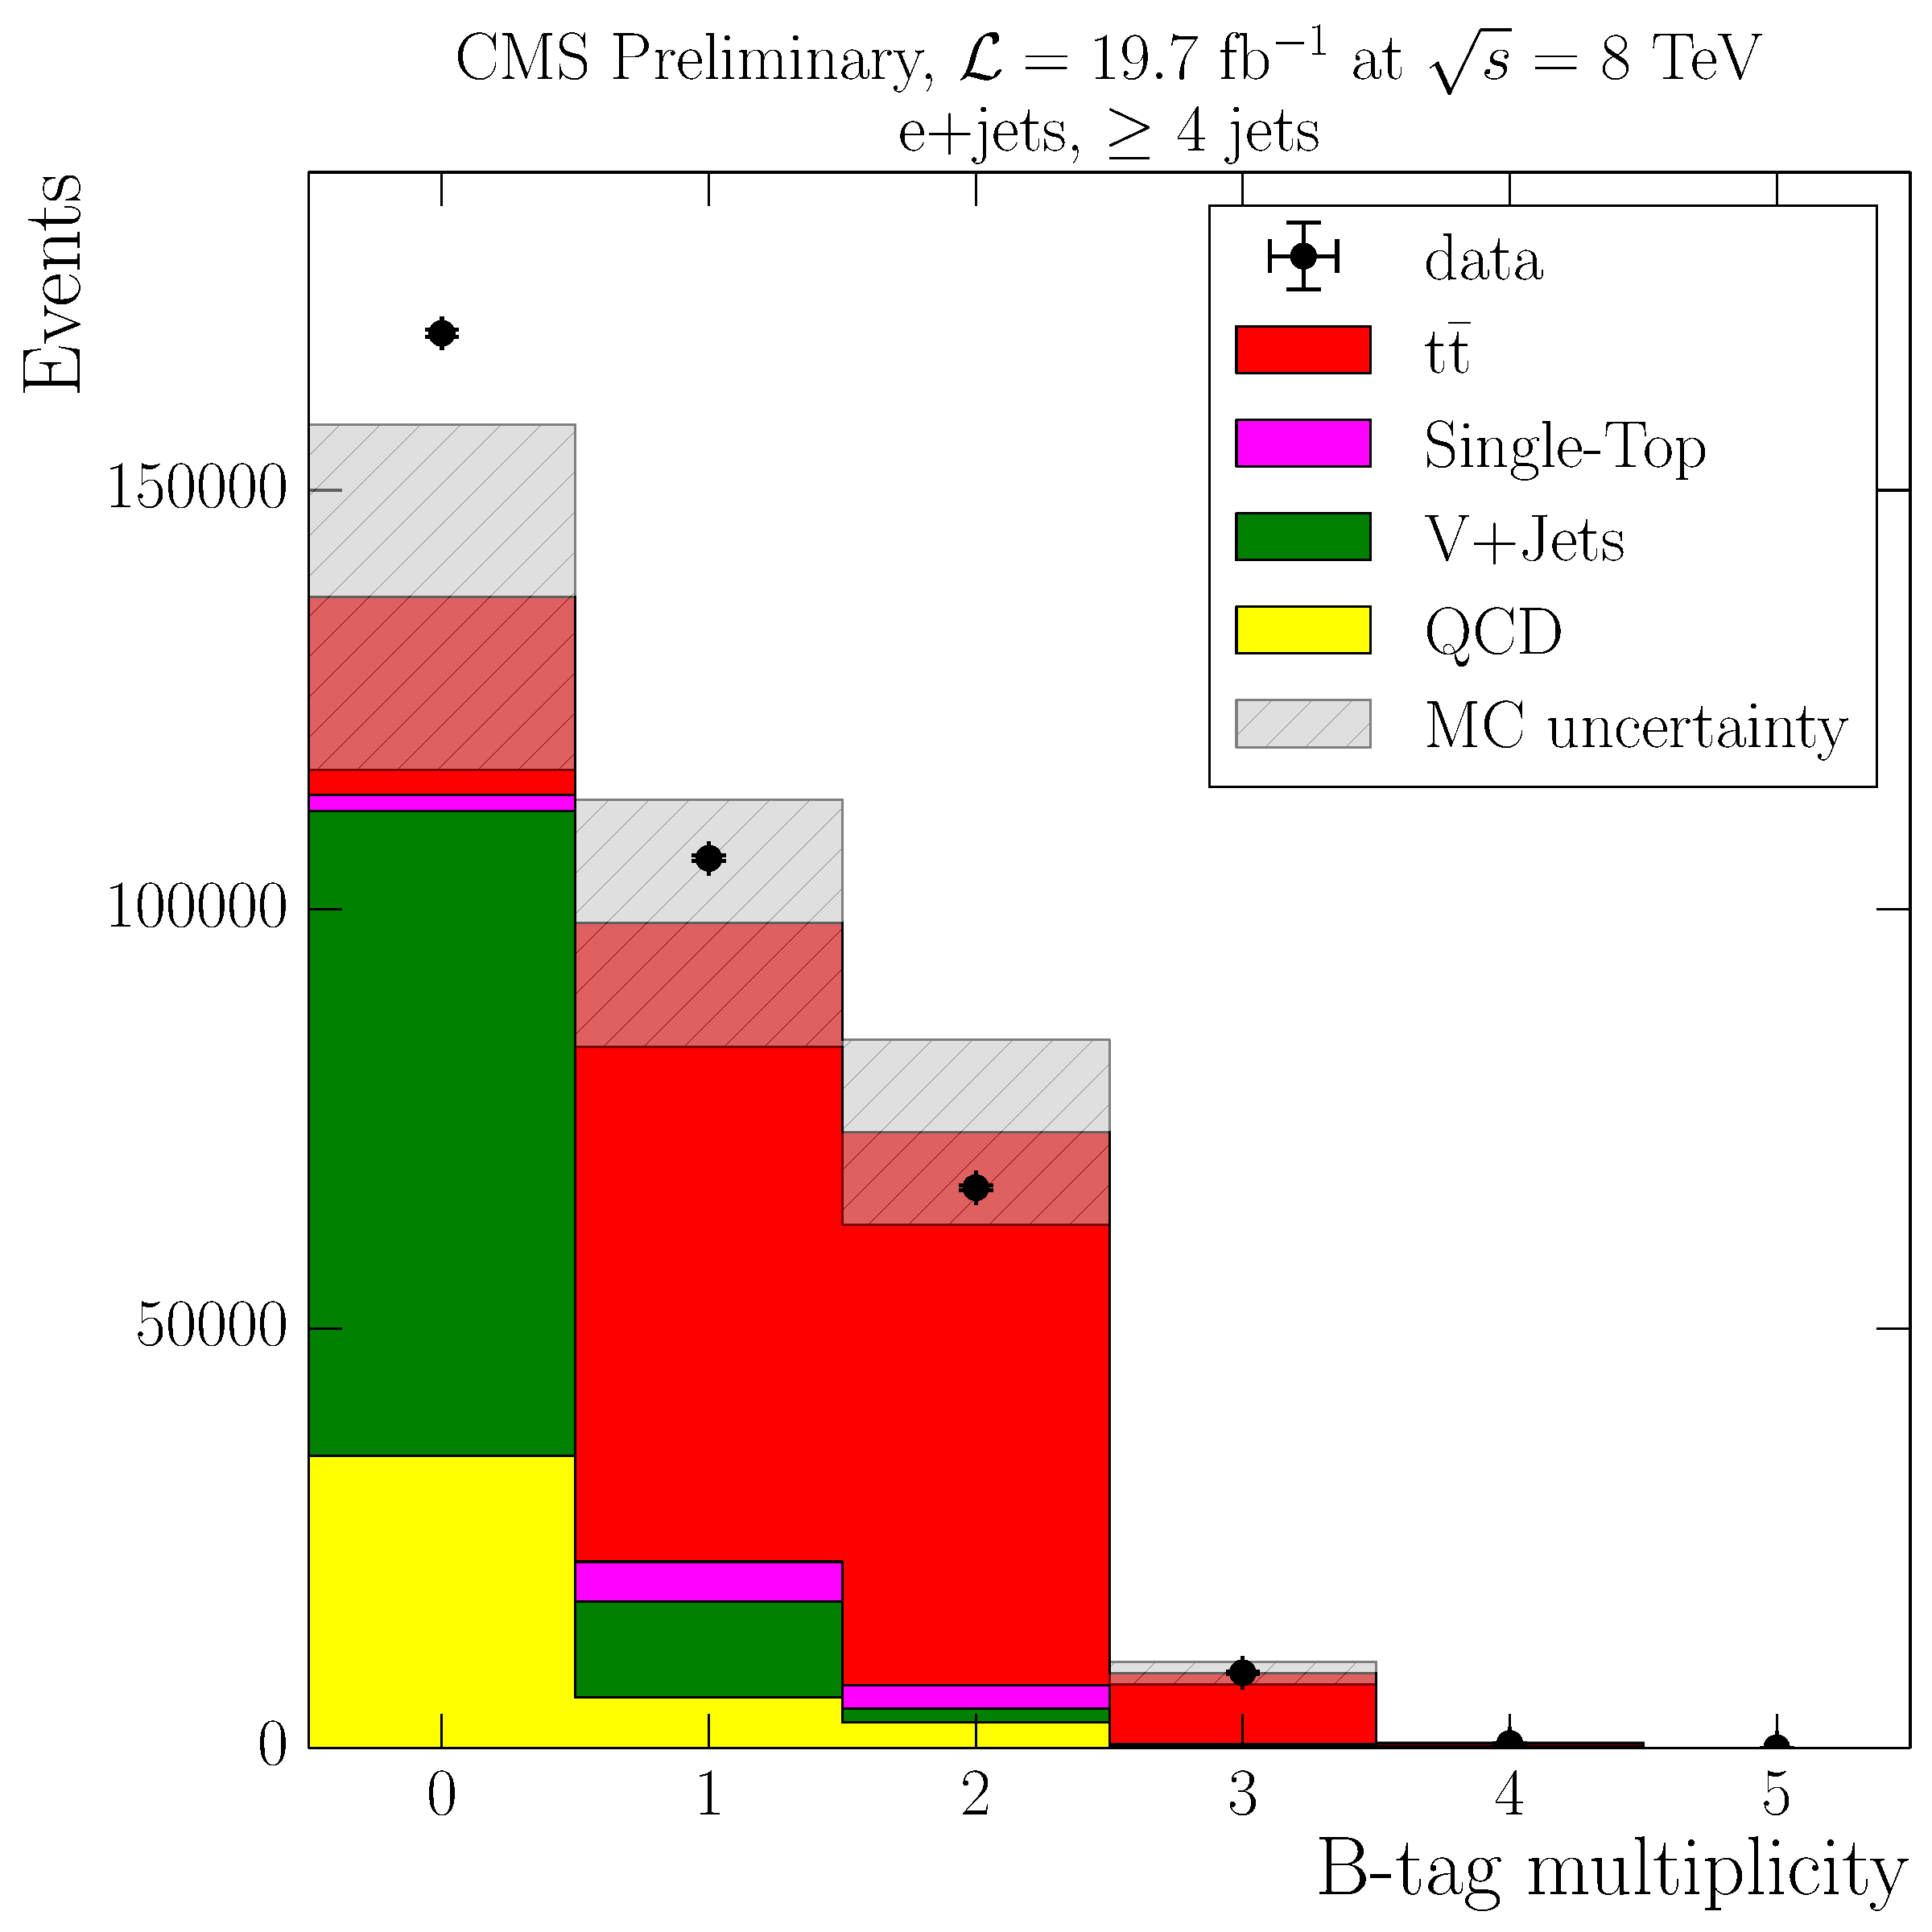
\includegraphics[width=0.50\textwidth]{bjets_multiplicity/EPlusJets_N_BJets.pdf}}\hfill
	\subfloat[]{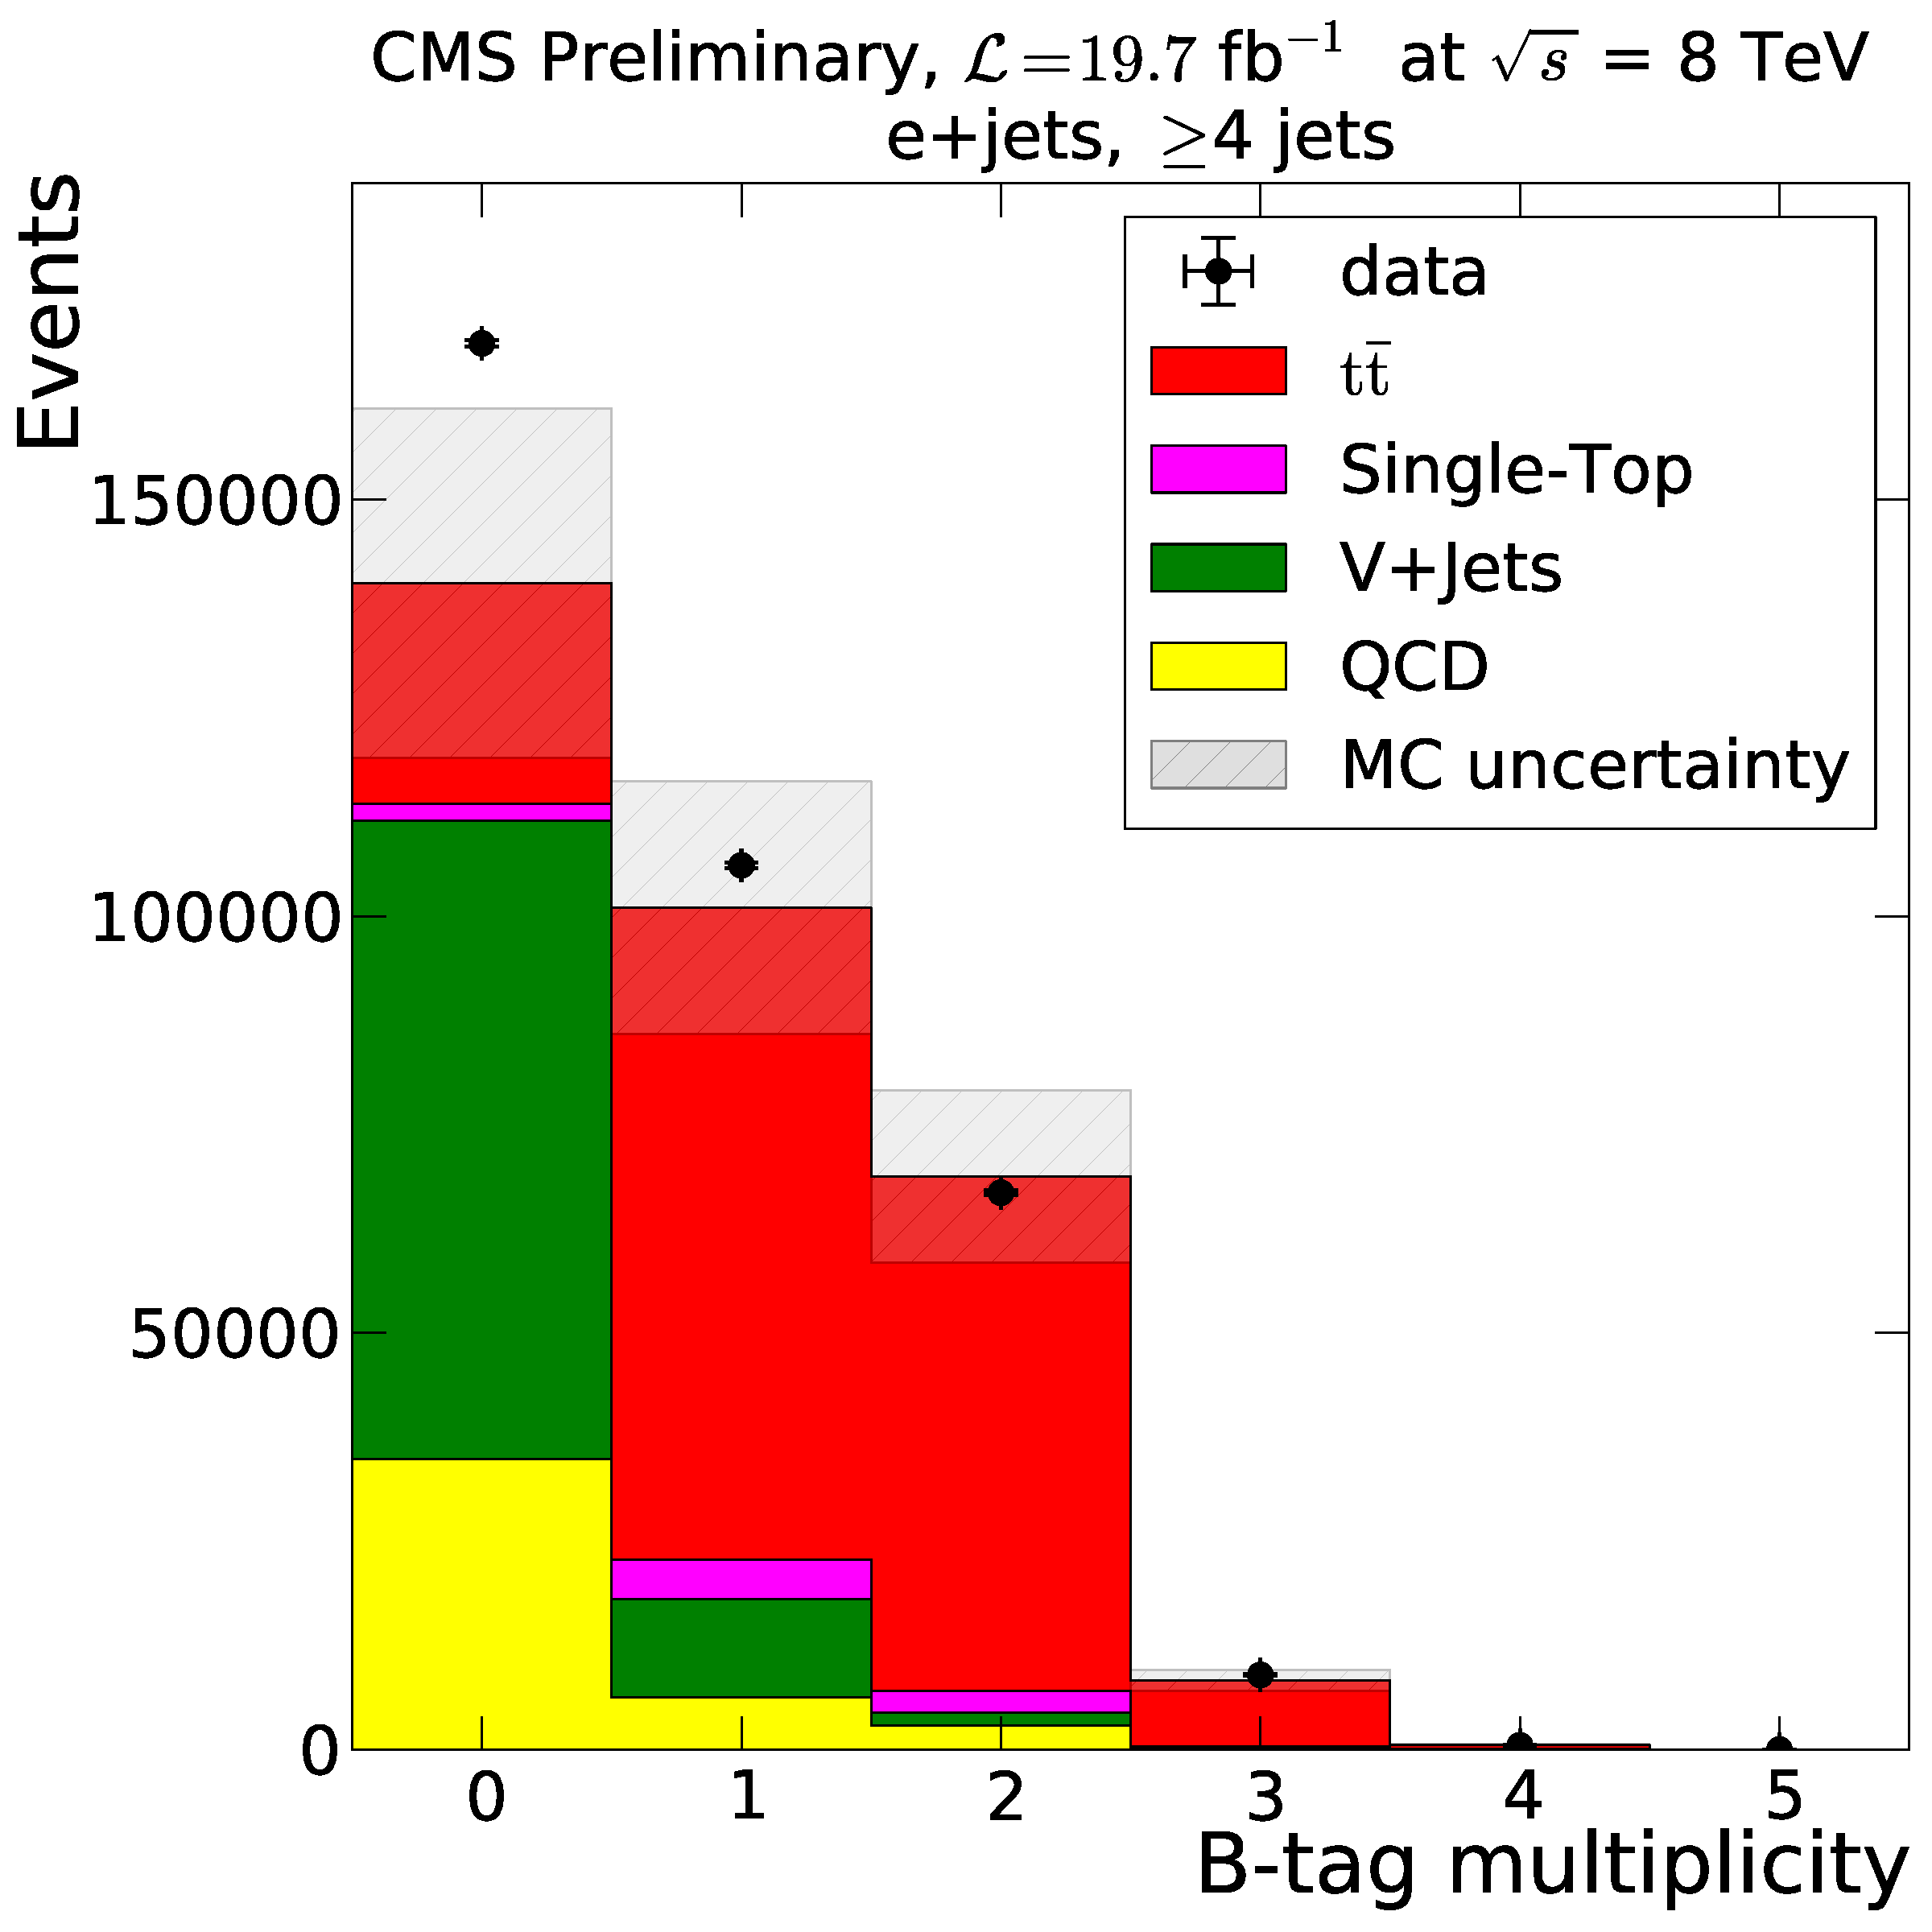
\includegraphics[width=0.50\textwidth]{bjets_multiplicity/EPlusJets_N_BJets_reweighted.pdf}} \\
	\subfloat[]{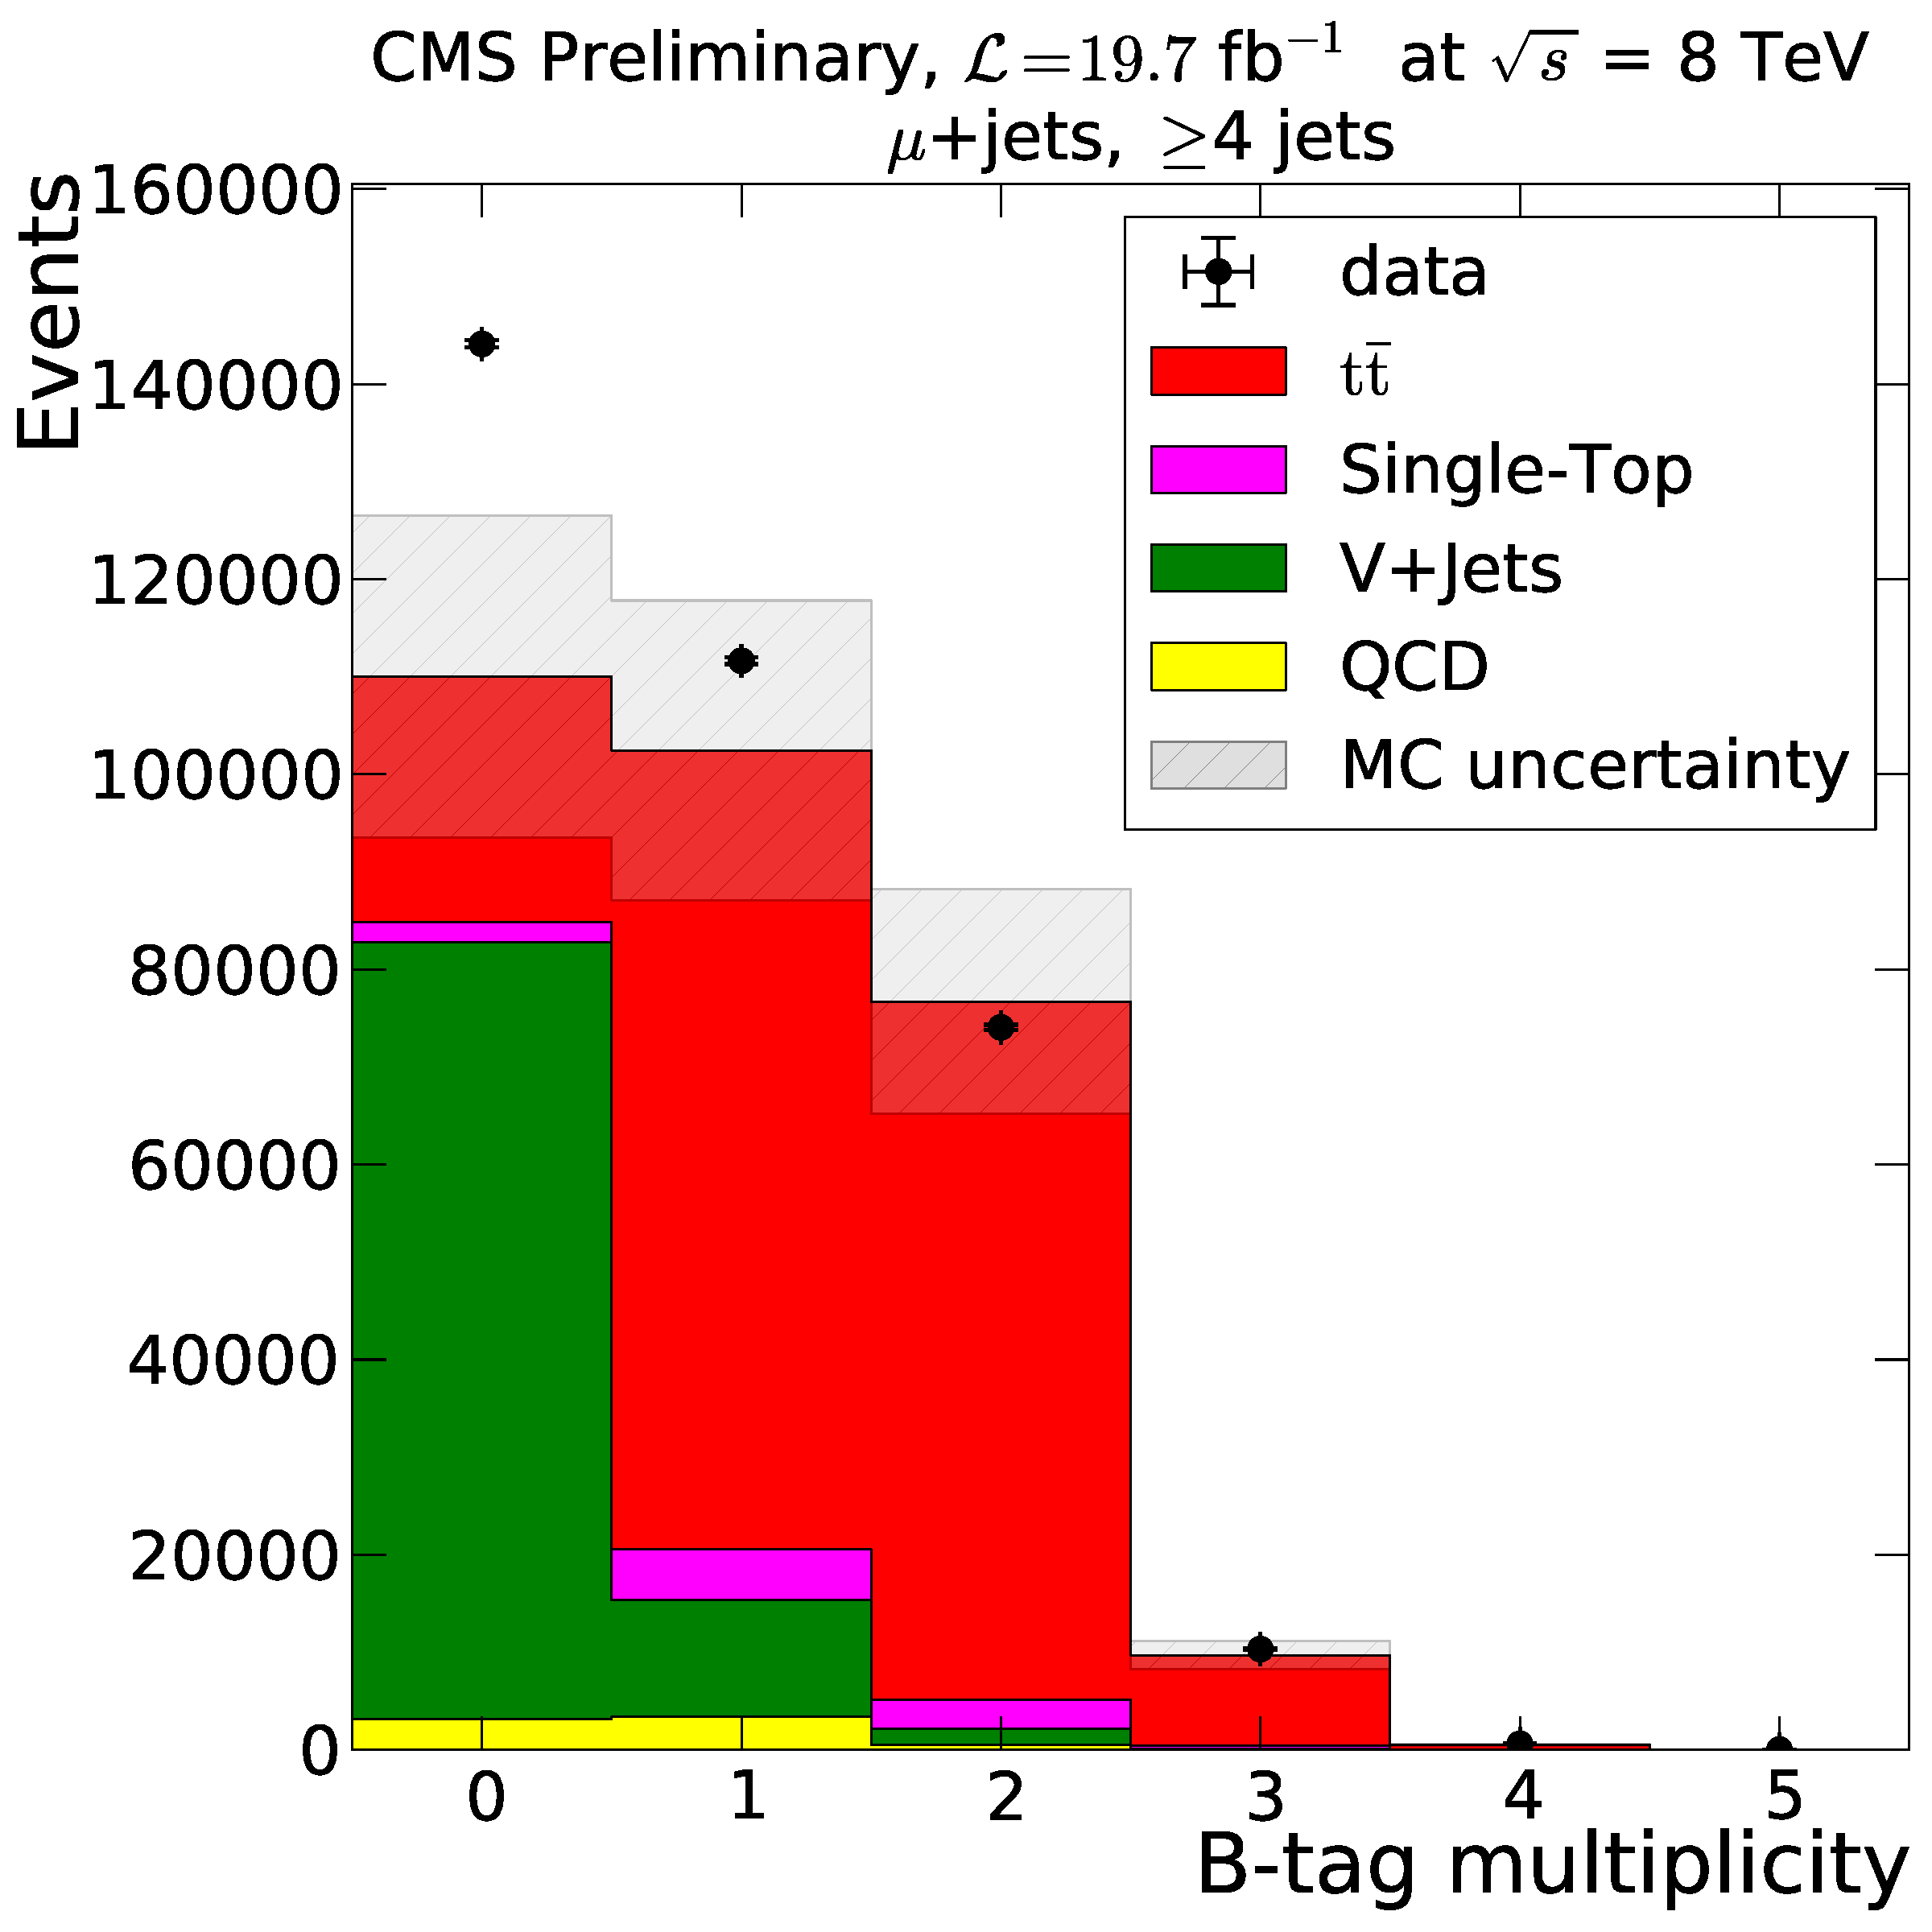
\includegraphics[width=0.50\textwidth]{bjets_multiplicity/MuPlusJets_N_BJets.pdf}}\hfill
	\subfloat[]{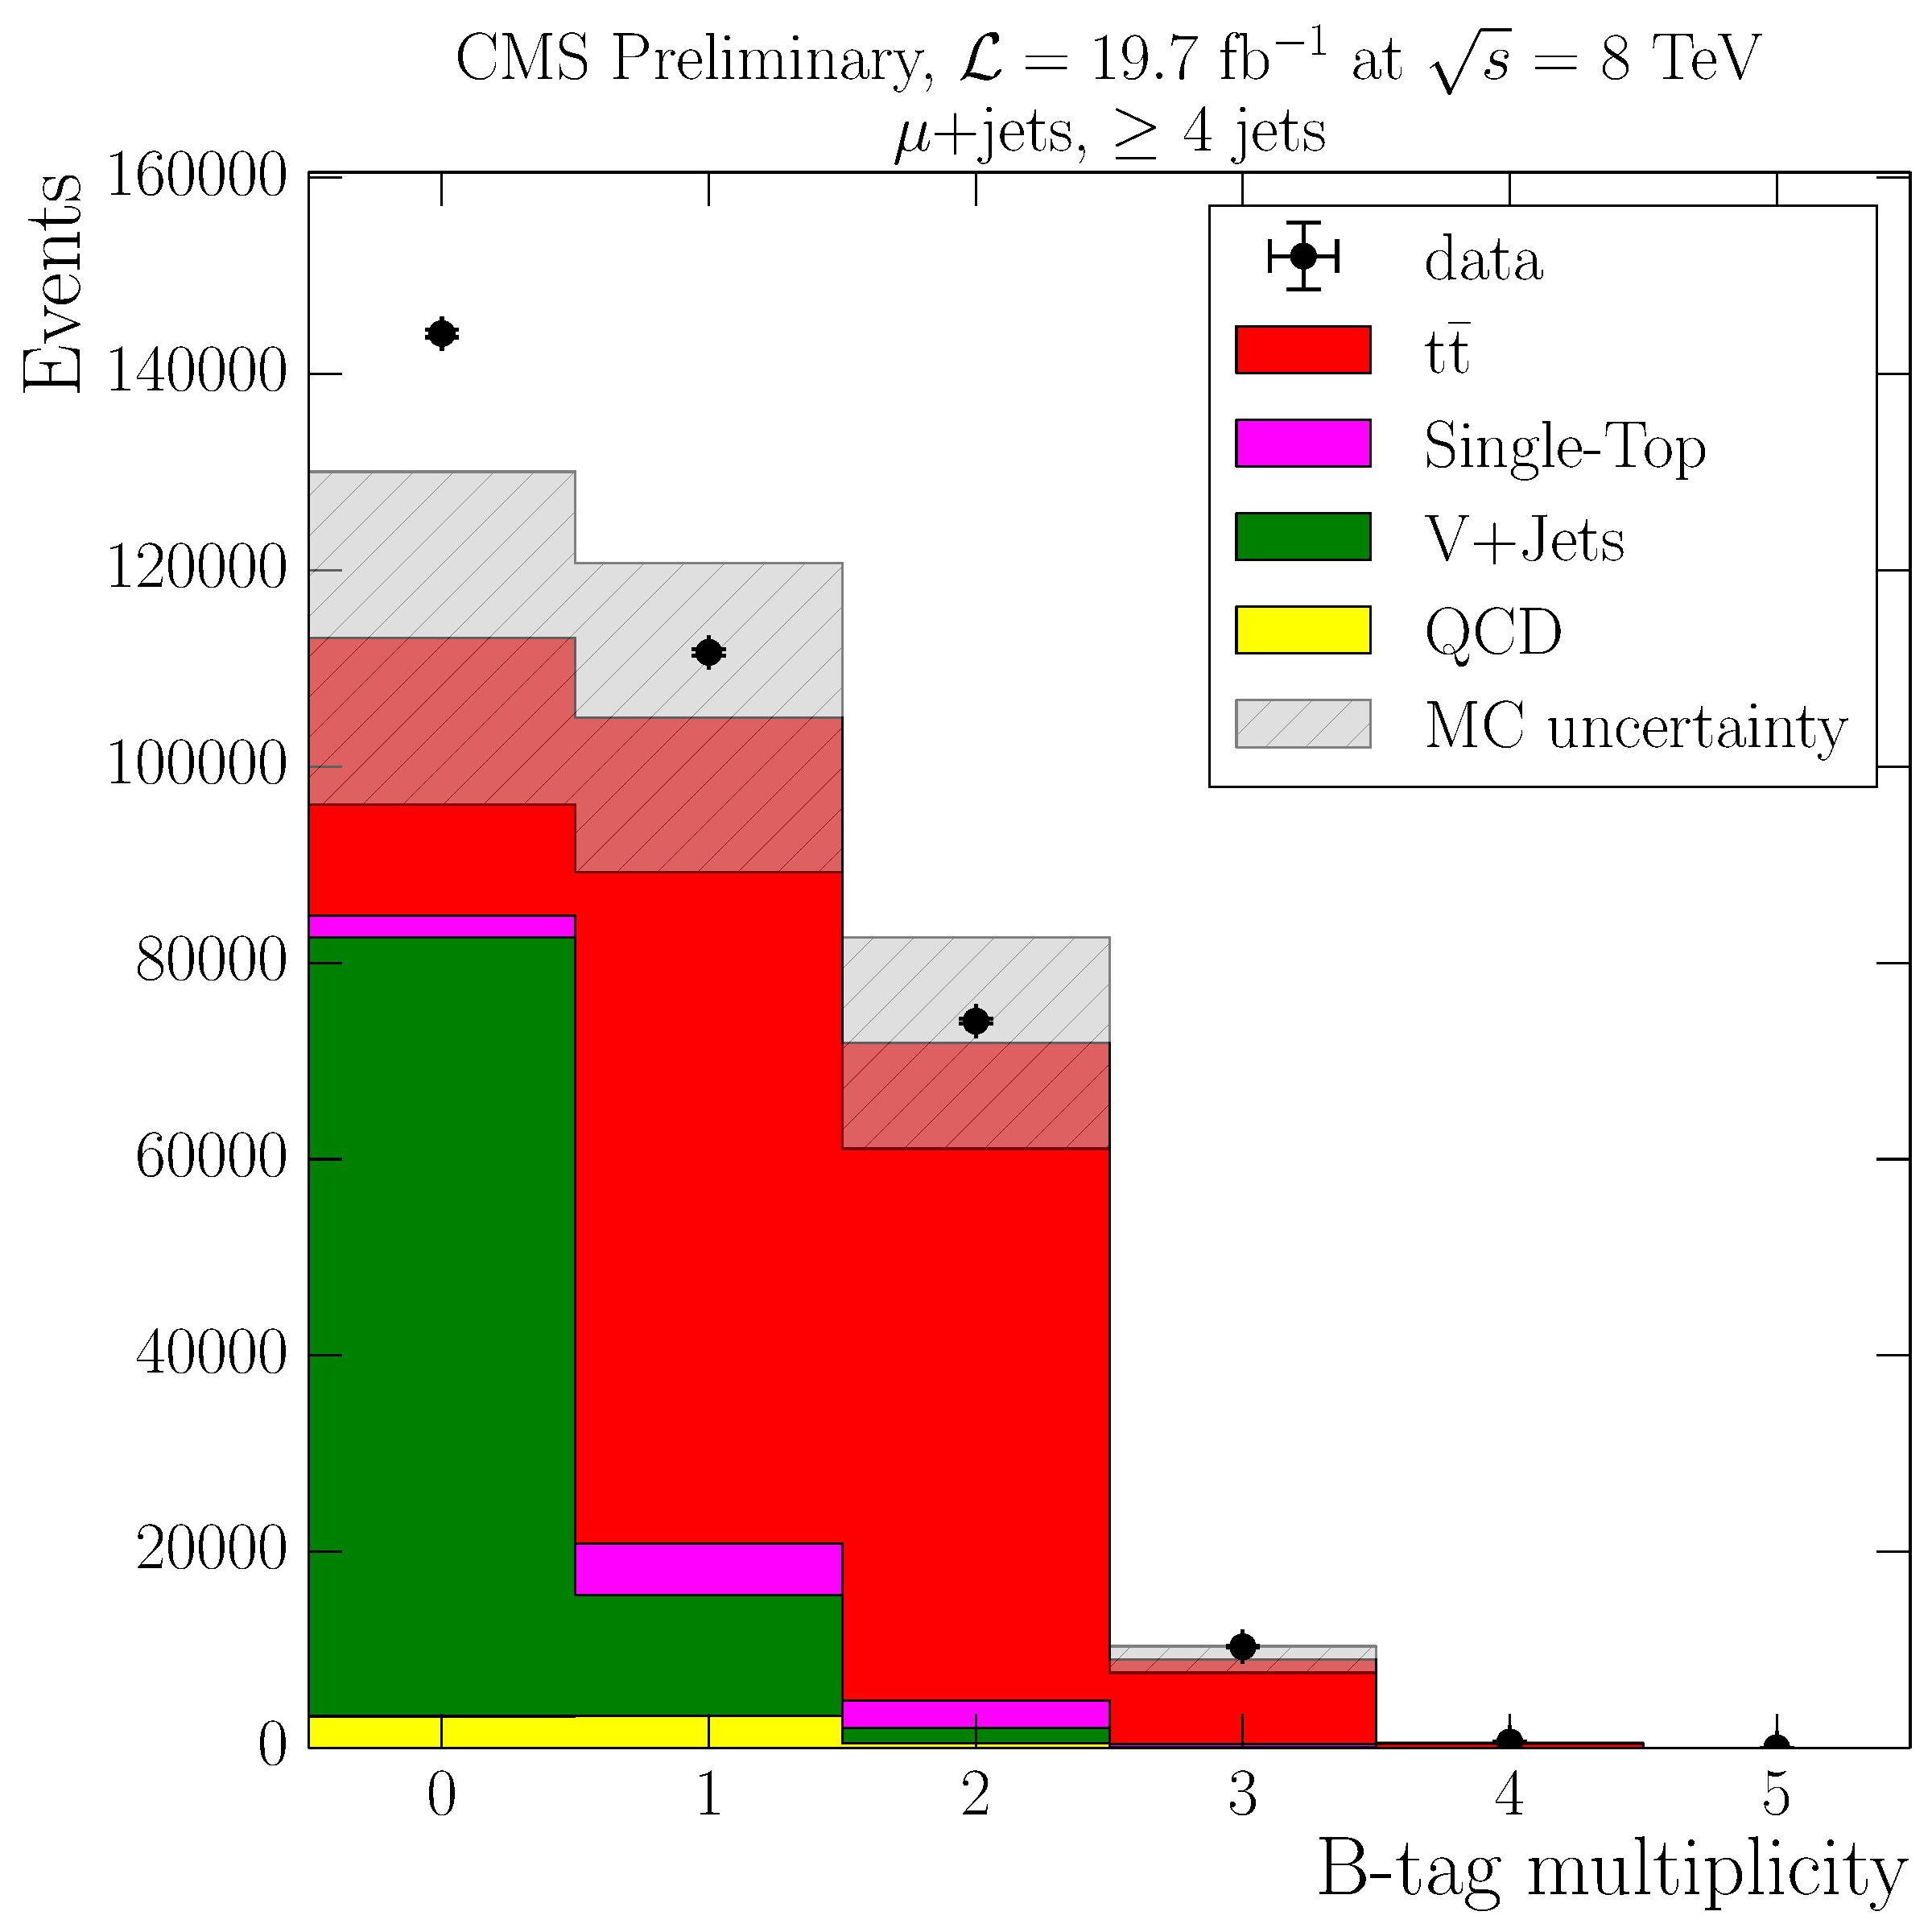
\includegraphics[width=0.50\textwidth]{bjets_multiplicity/MuPlusJets_N_BJets_reweighted.pdf}}
	\caption{\label{fig:bjet_weights}
    b-tag multiplicity before (left) and after applying b-tag scale factors (right) in the electron channel (top) and
    the muon channel (bottom).}
\end{center}
\end{figure}

\section{Event Selection}
\label{s_xsection:event_selection}

\section{Data-driven QCD estimation}
\label{s_xsection:data_driven_QCD}

\section{Choice of binning}
\label{s_xsection:binning}

\section{Differential cross section measurement}
\label{s_xsection:measurement}

\section{Unfolding}
\label{s_xsection:unfolding}

\section{Systematic Uncertainties}
\label{s_xsection:systematics}

\section{Results}
\label{s_xsection:results}

%%% Local Variables: 
%%% mode: latex
%%% TeX-master: "../thesis"
%%% End: 
